% !TEX root = ../sethomas_thesis_main.tex
\documentclass[border=1mm,
               class=article
               preview]{standalone}
\usepackage{tikz}
\begin{document}
\begin{tikzpicture}
    \node[anchor=south west,inner sep=0] (graph) at (0,0) {\resizebox{\columnwidth}{!}{%% Creator: Matplotlib, PGF backend
%%
%% To include the figure in your LaTeX document, write
%%   \input{<filename>.pgf}
%%
%% Make sure the required packages are loaded in your preamble
%%   \usepackage{pgf}
%%
%% and, on pdftex
%%   \usepackage[utf8]{inputenc}\DeclareUnicodeCharacter{2212}{-}
%%
%% or, on luatex and xetex
%%   \usepackage{unicode-math}
%%
%% Figures using additional raster images can only be included by \input if
%% they are in the same directory as the main LaTeX file. For loading figures
%% from other directories you can use the `import` package
%%   \usepackage{import}
%%
%% and then include the figures with
%%   \import{<path to file>}{<filename>.pgf}
%%
%% Matplotlib used the following preamble
%%
\begingroup%
\makeatletter%
\begin{pgfpicture}%
\pgfpathrectangle{\pgfpointorigin}{\pgfqpoint{8.602007in}{4.649344in}}%
\pgfusepath{use as bounding box, clip}%
\begin{pgfscope}%
\pgfsetbuttcap%
\pgfsetmiterjoin%
\pgfsetlinewidth{0.000000pt}%
\definecolor{currentstroke}{rgb}{0.000000,0.000000,0.000000}%
\pgfsetstrokecolor{currentstroke}%
\pgfsetstrokeopacity{0.000000}%
\pgfsetdash{}{0pt}%
\pgfpathmoveto{\pgfqpoint{0.000000in}{0.000000in}}%
\pgfpathlineto{\pgfqpoint{8.602007in}{0.000000in}}%
\pgfpathlineto{\pgfqpoint{8.602007in}{4.649344in}}%
\pgfpathlineto{\pgfqpoint{0.000000in}{4.649344in}}%
\pgfpathclose%
\pgfusepath{}%
\end{pgfscope}%
\begin{pgfscope}%
\pgfsetbuttcap%
\pgfsetmiterjoin%
\pgfsetlinewidth{0.000000pt}%
\definecolor{currentstroke}{rgb}{0.000000,0.000000,0.000000}%
\pgfsetstrokecolor{currentstroke}%
\pgfsetstrokeopacity{0.000000}%
\pgfsetdash{}{0pt}%
\pgfpathmoveto{\pgfqpoint{0.717284in}{3.271659in}}%
\pgfpathlineto{\pgfqpoint{8.467284in}{3.271659in}}%
\pgfpathlineto{\pgfqpoint{8.467284in}{4.404012in}}%
\pgfpathlineto{\pgfqpoint{0.717284in}{4.404012in}}%
\pgfpathclose%
\pgfusepath{}%
\end{pgfscope}%
\begin{pgfscope}%
\pgfpathrectangle{\pgfqpoint{0.717284in}{3.271659in}}{\pgfqpoint{7.750000in}{1.132353in}}%
\pgfusepath{clip}%
\pgfsetbuttcap%
\pgfsetroundjoin%
\pgfsetlinewidth{0.803000pt}%
\definecolor{currentstroke}{rgb}{0.690196,0.690196,0.690196}%
\pgfsetstrokecolor{currentstroke}%
\pgfsetdash{{2.960000pt}{1.280000pt}}{0.000000pt}%
\pgfpathmoveto{\pgfqpoint{2.654784in}{3.271659in}}%
\pgfpathlineto{\pgfqpoint{2.654784in}{4.404012in}}%
\pgfusepath{stroke}%
\end{pgfscope}%
\begin{pgfscope}%
\pgfsetbuttcap%
\pgfsetroundjoin%
\definecolor{currentfill}{rgb}{0.000000,0.000000,0.000000}%
\pgfsetfillcolor{currentfill}%
\pgfsetlinewidth{0.803000pt}%
\definecolor{currentstroke}{rgb}{0.000000,0.000000,0.000000}%
\pgfsetstrokecolor{currentstroke}%
\pgfsetdash{}{0pt}%
\pgfsys@defobject{currentmarker}{\pgfqpoint{0.000000in}{-0.048611in}}{\pgfqpoint{0.000000in}{0.000000in}}{%
\pgfpathmoveto{\pgfqpoint{0.000000in}{0.000000in}}%
\pgfpathlineto{\pgfqpoint{0.000000in}{-0.048611in}}%
\pgfusepath{stroke,fill}%
}%
\begin{pgfscope}%
\pgfsys@transformshift{2.654784in}{3.271659in}%
\pgfsys@useobject{currentmarker}{}%
\end{pgfscope}%
\end{pgfscope}%
\begin{pgfscope}%
\pgfpathrectangle{\pgfqpoint{0.717284in}{3.271659in}}{\pgfqpoint{7.750000in}{1.132353in}}%
\pgfusepath{clip}%
\pgfsetbuttcap%
\pgfsetroundjoin%
\pgfsetlinewidth{0.803000pt}%
\definecolor{currentstroke}{rgb}{0.690196,0.690196,0.690196}%
\pgfsetstrokecolor{currentstroke}%
\pgfsetdash{{2.960000pt}{1.280000pt}}{0.000000pt}%
\pgfpathmoveto{\pgfqpoint{4.592284in}{3.271659in}}%
\pgfpathlineto{\pgfqpoint{4.592284in}{4.404012in}}%
\pgfusepath{stroke}%
\end{pgfscope}%
\begin{pgfscope}%
\pgfsetbuttcap%
\pgfsetroundjoin%
\definecolor{currentfill}{rgb}{0.000000,0.000000,0.000000}%
\pgfsetfillcolor{currentfill}%
\pgfsetlinewidth{0.803000pt}%
\definecolor{currentstroke}{rgb}{0.000000,0.000000,0.000000}%
\pgfsetstrokecolor{currentstroke}%
\pgfsetdash{}{0pt}%
\pgfsys@defobject{currentmarker}{\pgfqpoint{0.000000in}{-0.048611in}}{\pgfqpoint{0.000000in}{0.000000in}}{%
\pgfpathmoveto{\pgfqpoint{0.000000in}{0.000000in}}%
\pgfpathlineto{\pgfqpoint{0.000000in}{-0.048611in}}%
\pgfusepath{stroke,fill}%
}%
\begin{pgfscope}%
\pgfsys@transformshift{4.592284in}{3.271659in}%
\pgfsys@useobject{currentmarker}{}%
\end{pgfscope}%
\end{pgfscope}%
\begin{pgfscope}%
\pgfpathrectangle{\pgfqpoint{0.717284in}{3.271659in}}{\pgfqpoint{7.750000in}{1.132353in}}%
\pgfusepath{clip}%
\pgfsetbuttcap%
\pgfsetroundjoin%
\pgfsetlinewidth{0.803000pt}%
\definecolor{currentstroke}{rgb}{0.690196,0.690196,0.690196}%
\pgfsetstrokecolor{currentstroke}%
\pgfsetdash{{2.960000pt}{1.280000pt}}{0.000000pt}%
\pgfpathmoveto{\pgfqpoint{6.529784in}{3.271659in}}%
\pgfpathlineto{\pgfqpoint{6.529784in}{4.404012in}}%
\pgfusepath{stroke}%
\end{pgfscope}%
\begin{pgfscope}%
\pgfsetbuttcap%
\pgfsetroundjoin%
\definecolor{currentfill}{rgb}{0.000000,0.000000,0.000000}%
\pgfsetfillcolor{currentfill}%
\pgfsetlinewidth{0.803000pt}%
\definecolor{currentstroke}{rgb}{0.000000,0.000000,0.000000}%
\pgfsetstrokecolor{currentstroke}%
\pgfsetdash{}{0pt}%
\pgfsys@defobject{currentmarker}{\pgfqpoint{0.000000in}{-0.048611in}}{\pgfqpoint{0.000000in}{0.000000in}}{%
\pgfpathmoveto{\pgfqpoint{0.000000in}{0.000000in}}%
\pgfpathlineto{\pgfqpoint{0.000000in}{-0.048611in}}%
\pgfusepath{stroke,fill}%
}%
\begin{pgfscope}%
\pgfsys@transformshift{6.529784in}{3.271659in}%
\pgfsys@useobject{currentmarker}{}%
\end{pgfscope}%
\end{pgfscope}%
\begin{pgfscope}%
\pgfpathrectangle{\pgfqpoint{0.717284in}{3.271659in}}{\pgfqpoint{7.750000in}{1.132353in}}%
\pgfusepath{clip}%
\pgfsetbuttcap%
\pgfsetroundjoin%
\pgfsetlinewidth{0.803000pt}%
\definecolor{currentstroke}{rgb}{0.690196,0.690196,0.690196}%
\pgfsetstrokecolor{currentstroke}%
\pgfsetdash{{2.960000pt}{1.280000pt}}{0.000000pt}%
\pgfpathmoveto{\pgfqpoint{8.467284in}{3.271659in}}%
\pgfpathlineto{\pgfqpoint{8.467284in}{4.404012in}}%
\pgfusepath{stroke}%
\end{pgfscope}%
\begin{pgfscope}%
\pgfsetbuttcap%
\pgfsetroundjoin%
\definecolor{currentfill}{rgb}{0.000000,0.000000,0.000000}%
\pgfsetfillcolor{currentfill}%
\pgfsetlinewidth{0.803000pt}%
\definecolor{currentstroke}{rgb}{0.000000,0.000000,0.000000}%
\pgfsetstrokecolor{currentstroke}%
\pgfsetdash{}{0pt}%
\pgfsys@defobject{currentmarker}{\pgfqpoint{0.000000in}{-0.048611in}}{\pgfqpoint{0.000000in}{0.000000in}}{%
\pgfpathmoveto{\pgfqpoint{0.000000in}{0.000000in}}%
\pgfpathlineto{\pgfqpoint{0.000000in}{-0.048611in}}%
\pgfusepath{stroke,fill}%
}%
\begin{pgfscope}%
\pgfsys@transformshift{8.467284in}{3.271659in}%
\pgfsys@useobject{currentmarker}{}%
\end{pgfscope}%
\end{pgfscope}%
\begin{pgfscope}%
\pgfpathrectangle{\pgfqpoint{0.717284in}{3.271659in}}{\pgfqpoint{7.750000in}{1.132353in}}%
\pgfusepath{clip}%
\pgfsetbuttcap%
\pgfsetroundjoin%
\pgfsetlinewidth{0.803000pt}%
\definecolor{currentstroke}{rgb}{0.690196,0.690196,0.690196}%
\pgfsetstrokecolor{currentstroke}%
\pgfsetdash{{2.960000pt}{1.280000pt}}{0.000000pt}%
\pgfpathmoveto{\pgfqpoint{0.717284in}{3.323129in}}%
\pgfpathlineto{\pgfqpoint{8.467284in}{3.323129in}}%
\pgfusepath{stroke}%
\end{pgfscope}%
\begin{pgfscope}%
\pgfsetbuttcap%
\pgfsetroundjoin%
\definecolor{currentfill}{rgb}{0.000000,0.000000,0.000000}%
\pgfsetfillcolor{currentfill}%
\pgfsetlinewidth{0.803000pt}%
\definecolor{currentstroke}{rgb}{0.000000,0.000000,0.000000}%
\pgfsetstrokecolor{currentstroke}%
\pgfsetdash{}{0pt}%
\pgfsys@defobject{currentmarker}{\pgfqpoint{-0.048611in}{0.000000in}}{\pgfqpoint{-0.000000in}{0.000000in}}{%
\pgfpathmoveto{\pgfqpoint{-0.000000in}{0.000000in}}%
\pgfpathlineto{\pgfqpoint{-0.048611in}{0.000000in}}%
\pgfusepath{stroke,fill}%
}%
\begin{pgfscope}%
\pgfsys@transformshift{0.717284in}{3.323129in}%
\pgfsys@useobject{currentmarker}{}%
\end{pgfscope}%
\end{pgfscope}%
\begin{pgfscope}%
\definecolor{textcolor}{rgb}{0.000000,0.000000,0.000000}%
\pgfsetstrokecolor{textcolor}%
\pgfsetfillcolor{textcolor}%
\pgftext[x=0.481173in, y=3.274904in, left, base]{\color{textcolor}\rmfamily\fontsize{10.000000}{12.000000}\selectfont \(\displaystyle {22}\)}%
\end{pgfscope}%
\begin{pgfscope}%
\pgfpathrectangle{\pgfqpoint{0.717284in}{3.271659in}}{\pgfqpoint{7.750000in}{1.132353in}}%
\pgfusepath{clip}%
\pgfsetbuttcap%
\pgfsetroundjoin%
\pgfsetlinewidth{0.803000pt}%
\definecolor{currentstroke}{rgb}{0.690196,0.690196,0.690196}%
\pgfsetstrokecolor{currentstroke}%
\pgfsetdash{{2.960000pt}{1.280000pt}}{0.000000pt}%
\pgfpathmoveto{\pgfqpoint{0.717284in}{4.352541in}}%
\pgfpathlineto{\pgfqpoint{8.467284in}{4.352541in}}%
\pgfusepath{stroke}%
\end{pgfscope}%
\begin{pgfscope}%
\pgfsetbuttcap%
\pgfsetroundjoin%
\definecolor{currentfill}{rgb}{0.000000,0.000000,0.000000}%
\pgfsetfillcolor{currentfill}%
\pgfsetlinewidth{0.803000pt}%
\definecolor{currentstroke}{rgb}{0.000000,0.000000,0.000000}%
\pgfsetstrokecolor{currentstroke}%
\pgfsetdash{}{0pt}%
\pgfsys@defobject{currentmarker}{\pgfqpoint{-0.048611in}{0.000000in}}{\pgfqpoint{-0.000000in}{0.000000in}}{%
\pgfpathmoveto{\pgfqpoint{-0.000000in}{0.000000in}}%
\pgfpathlineto{\pgfqpoint{-0.048611in}{0.000000in}}%
\pgfusepath{stroke,fill}%
}%
\begin{pgfscope}%
\pgfsys@transformshift{0.717284in}{4.352541in}%
\pgfsys@useobject{currentmarker}{}%
\end{pgfscope}%
\end{pgfscope}%
\begin{pgfscope}%
\definecolor{textcolor}{rgb}{0.000000,0.000000,0.000000}%
\pgfsetstrokecolor{textcolor}%
\pgfsetfillcolor{textcolor}%
\pgftext[x=0.411728in, y=4.304316in, left, base]{\color{textcolor}\rmfamily\fontsize{10.000000}{12.000000}\selectfont \(\displaystyle {160}\)}%
\end{pgfscope}%
\begin{pgfscope}%
\definecolor{textcolor}{rgb}{0.000000,0.000000,0.000000}%
\pgfsetstrokecolor{textcolor}%
\pgfsetfillcolor{textcolor}%
\pgftext[x=0.356173in,y=3.837835in,,bottom,rotate=90.000000]{\color{textcolor}\rmfamily\fontsize{12.000000}{14.400000}\bfseries\selectfont Temperature [°C]}%
\end{pgfscope}%
\begin{pgfscope}%
\pgfpathrectangle{\pgfqpoint{0.717284in}{3.271659in}}{\pgfqpoint{7.750000in}{1.132353in}}%
\pgfusepath{clip}%
\pgfsetbuttcap%
\pgfsetroundjoin%
\pgfsetlinewidth{3.011250pt}%
\definecolor{currentstroke}{rgb}{0.450980,0.670588,1.000000}%
\pgfsetstrokecolor{currentstroke}%
\pgfsetdash{{3.000000pt}{4.950000pt}}{0.000000pt}%
\pgfpathmoveto{\pgfqpoint{0.717284in}{3.323129in}}%
\pgfpathlineto{\pgfqpoint{4.592284in}{3.323129in}}%
\pgfpathlineto{\pgfqpoint{5.756528in}{3.941672in}}%
\pgfpathlineto{\pgfqpoint{5.756916in}{3.941672in}}%
\pgfpathlineto{\pgfqpoint{6.529784in}{4.352541in}}%
\pgfpathlineto{\pgfqpoint{8.467284in}{3.323129in}}%
\pgfpathlineto{\pgfqpoint{8.467284in}{3.323129in}}%
\pgfusepath{stroke}%
\end{pgfscope}%
\begin{pgfscope}%
\pgfsetrectcap%
\pgfsetmiterjoin%
\pgfsetlinewidth{0.803000pt}%
\definecolor{currentstroke}{rgb}{0.000000,0.000000,0.000000}%
\pgfsetstrokecolor{currentstroke}%
\pgfsetdash{}{0pt}%
\pgfpathmoveto{\pgfqpoint{0.717284in}{3.271659in}}%
\pgfpathlineto{\pgfqpoint{0.717284in}{4.404012in}}%
\pgfusepath{stroke}%
\end{pgfscope}%
\begin{pgfscope}%
\pgfsetrectcap%
\pgfsetmiterjoin%
\pgfsetlinewidth{0.803000pt}%
\definecolor{currentstroke}{rgb}{0.000000,0.000000,0.000000}%
\pgfsetstrokecolor{currentstroke}%
\pgfsetdash{}{0pt}%
\pgfpathmoveto{\pgfqpoint{8.467284in}{3.271659in}}%
\pgfpathlineto{\pgfqpoint{8.467284in}{4.404012in}}%
\pgfusepath{stroke}%
\end{pgfscope}%
\begin{pgfscope}%
\pgfsetrectcap%
\pgfsetmiterjoin%
\pgfsetlinewidth{0.803000pt}%
\definecolor{currentstroke}{rgb}{0.000000,0.000000,0.000000}%
\pgfsetstrokecolor{currentstroke}%
\pgfsetdash{}{0pt}%
\pgfpathmoveto{\pgfqpoint{0.717284in}{3.271659in}}%
\pgfpathlineto{\pgfqpoint{8.467284in}{3.271659in}}%
\pgfusepath{stroke}%
\end{pgfscope}%
\begin{pgfscope}%
\pgfsetrectcap%
\pgfsetmiterjoin%
\pgfsetlinewidth{0.803000pt}%
\definecolor{currentstroke}{rgb}{0.000000,0.000000,0.000000}%
\pgfsetstrokecolor{currentstroke}%
\pgfsetdash{}{0pt}%
\pgfpathmoveto{\pgfqpoint{0.717284in}{4.404012in}}%
\pgfpathlineto{\pgfqpoint{8.467284in}{4.404012in}}%
\pgfusepath{stroke}%
\end{pgfscope}%
\begin{pgfscope}%
\pgfsetbuttcap%
\pgfsetmiterjoin%
\pgfsetlinewidth{0.000000pt}%
\definecolor{currentstroke}{rgb}{0.000000,0.000000,0.000000}%
\pgfsetstrokecolor{currentstroke}%
\pgfsetstrokeopacity{0.000000}%
\pgfsetdash{}{0pt}%
\pgfpathmoveto{\pgfqpoint{0.717284in}{1.912835in}}%
\pgfpathlineto{\pgfqpoint{8.467284in}{1.912835in}}%
\pgfpathlineto{\pgfqpoint{8.467284in}{3.045188in}}%
\pgfpathlineto{\pgfqpoint{0.717284in}{3.045188in}}%
\pgfpathclose%
\pgfusepath{}%
\end{pgfscope}%
\begin{pgfscope}%
\pgfpathrectangle{\pgfqpoint{0.717284in}{1.912835in}}{\pgfqpoint{7.750000in}{1.132353in}}%
\pgfusepath{clip}%
\pgfsetbuttcap%
\pgfsetroundjoin%
\pgfsetlinewidth{0.803000pt}%
\definecolor{currentstroke}{rgb}{0.690196,0.690196,0.690196}%
\pgfsetstrokecolor{currentstroke}%
\pgfsetdash{{2.960000pt}{1.280000pt}}{0.000000pt}%
\pgfpathmoveto{\pgfqpoint{2.654784in}{1.912835in}}%
\pgfpathlineto{\pgfqpoint{2.654784in}{3.045188in}}%
\pgfusepath{stroke}%
\end{pgfscope}%
\begin{pgfscope}%
\pgfsetbuttcap%
\pgfsetroundjoin%
\definecolor{currentfill}{rgb}{0.000000,0.000000,0.000000}%
\pgfsetfillcolor{currentfill}%
\pgfsetlinewidth{0.803000pt}%
\definecolor{currentstroke}{rgb}{0.000000,0.000000,0.000000}%
\pgfsetstrokecolor{currentstroke}%
\pgfsetdash{}{0pt}%
\pgfsys@defobject{currentmarker}{\pgfqpoint{0.000000in}{-0.048611in}}{\pgfqpoint{0.000000in}{0.000000in}}{%
\pgfpathmoveto{\pgfqpoint{0.000000in}{0.000000in}}%
\pgfpathlineto{\pgfqpoint{0.000000in}{-0.048611in}}%
\pgfusepath{stroke,fill}%
}%
\begin{pgfscope}%
\pgfsys@transformshift{2.654784in}{1.912835in}%
\pgfsys@useobject{currentmarker}{}%
\end{pgfscope}%
\end{pgfscope}%
\begin{pgfscope}%
\pgfpathrectangle{\pgfqpoint{0.717284in}{1.912835in}}{\pgfqpoint{7.750000in}{1.132353in}}%
\pgfusepath{clip}%
\pgfsetbuttcap%
\pgfsetroundjoin%
\pgfsetlinewidth{0.803000pt}%
\definecolor{currentstroke}{rgb}{0.690196,0.690196,0.690196}%
\pgfsetstrokecolor{currentstroke}%
\pgfsetdash{{2.960000pt}{1.280000pt}}{0.000000pt}%
\pgfpathmoveto{\pgfqpoint{4.592284in}{1.912835in}}%
\pgfpathlineto{\pgfqpoint{4.592284in}{3.045188in}}%
\pgfusepath{stroke}%
\end{pgfscope}%
\begin{pgfscope}%
\pgfsetbuttcap%
\pgfsetroundjoin%
\definecolor{currentfill}{rgb}{0.000000,0.000000,0.000000}%
\pgfsetfillcolor{currentfill}%
\pgfsetlinewidth{0.803000pt}%
\definecolor{currentstroke}{rgb}{0.000000,0.000000,0.000000}%
\pgfsetstrokecolor{currentstroke}%
\pgfsetdash{}{0pt}%
\pgfsys@defobject{currentmarker}{\pgfqpoint{0.000000in}{-0.048611in}}{\pgfqpoint{0.000000in}{0.000000in}}{%
\pgfpathmoveto{\pgfqpoint{0.000000in}{0.000000in}}%
\pgfpathlineto{\pgfqpoint{0.000000in}{-0.048611in}}%
\pgfusepath{stroke,fill}%
}%
\begin{pgfscope}%
\pgfsys@transformshift{4.592284in}{1.912835in}%
\pgfsys@useobject{currentmarker}{}%
\end{pgfscope}%
\end{pgfscope}%
\begin{pgfscope}%
\pgfpathrectangle{\pgfqpoint{0.717284in}{1.912835in}}{\pgfqpoint{7.750000in}{1.132353in}}%
\pgfusepath{clip}%
\pgfsetbuttcap%
\pgfsetroundjoin%
\pgfsetlinewidth{0.803000pt}%
\definecolor{currentstroke}{rgb}{0.690196,0.690196,0.690196}%
\pgfsetstrokecolor{currentstroke}%
\pgfsetdash{{2.960000pt}{1.280000pt}}{0.000000pt}%
\pgfpathmoveto{\pgfqpoint{6.529784in}{1.912835in}}%
\pgfpathlineto{\pgfqpoint{6.529784in}{3.045188in}}%
\pgfusepath{stroke}%
\end{pgfscope}%
\begin{pgfscope}%
\pgfsetbuttcap%
\pgfsetroundjoin%
\definecolor{currentfill}{rgb}{0.000000,0.000000,0.000000}%
\pgfsetfillcolor{currentfill}%
\pgfsetlinewidth{0.803000pt}%
\definecolor{currentstroke}{rgb}{0.000000,0.000000,0.000000}%
\pgfsetstrokecolor{currentstroke}%
\pgfsetdash{}{0pt}%
\pgfsys@defobject{currentmarker}{\pgfqpoint{0.000000in}{-0.048611in}}{\pgfqpoint{0.000000in}{0.000000in}}{%
\pgfpathmoveto{\pgfqpoint{0.000000in}{0.000000in}}%
\pgfpathlineto{\pgfqpoint{0.000000in}{-0.048611in}}%
\pgfusepath{stroke,fill}%
}%
\begin{pgfscope}%
\pgfsys@transformshift{6.529784in}{1.912835in}%
\pgfsys@useobject{currentmarker}{}%
\end{pgfscope}%
\end{pgfscope}%
\begin{pgfscope}%
\pgfpathrectangle{\pgfqpoint{0.717284in}{1.912835in}}{\pgfqpoint{7.750000in}{1.132353in}}%
\pgfusepath{clip}%
\pgfsetbuttcap%
\pgfsetroundjoin%
\pgfsetlinewidth{0.803000pt}%
\definecolor{currentstroke}{rgb}{0.690196,0.690196,0.690196}%
\pgfsetstrokecolor{currentstroke}%
\pgfsetdash{{2.960000pt}{1.280000pt}}{0.000000pt}%
\pgfpathmoveto{\pgfqpoint{8.467284in}{1.912835in}}%
\pgfpathlineto{\pgfqpoint{8.467284in}{3.045188in}}%
\pgfusepath{stroke}%
\end{pgfscope}%
\begin{pgfscope}%
\pgfsetbuttcap%
\pgfsetroundjoin%
\definecolor{currentfill}{rgb}{0.000000,0.000000,0.000000}%
\pgfsetfillcolor{currentfill}%
\pgfsetlinewidth{0.803000pt}%
\definecolor{currentstroke}{rgb}{0.000000,0.000000,0.000000}%
\pgfsetstrokecolor{currentstroke}%
\pgfsetdash{}{0pt}%
\pgfsys@defobject{currentmarker}{\pgfqpoint{0.000000in}{-0.048611in}}{\pgfqpoint{0.000000in}{0.000000in}}{%
\pgfpathmoveto{\pgfqpoint{0.000000in}{0.000000in}}%
\pgfpathlineto{\pgfqpoint{0.000000in}{-0.048611in}}%
\pgfusepath{stroke,fill}%
}%
\begin{pgfscope}%
\pgfsys@transformshift{8.467284in}{1.912835in}%
\pgfsys@useobject{currentmarker}{}%
\end{pgfscope}%
\end{pgfscope}%
\begin{pgfscope}%
\pgfpathrectangle{\pgfqpoint{0.717284in}{1.912835in}}{\pgfqpoint{7.750000in}{1.132353in}}%
\pgfusepath{clip}%
\pgfsetbuttcap%
\pgfsetroundjoin%
\pgfsetlinewidth{0.803000pt}%
\definecolor{currentstroke}{rgb}{0.690196,0.690196,0.690196}%
\pgfsetstrokecolor{currentstroke}%
\pgfsetdash{{2.960000pt}{1.280000pt}}{0.000000pt}%
\pgfpathmoveto{\pgfqpoint{0.717284in}{1.964306in}}%
\pgfpathlineto{\pgfqpoint{8.467284in}{1.964306in}}%
\pgfusepath{stroke}%
\end{pgfscope}%
\begin{pgfscope}%
\pgfsetbuttcap%
\pgfsetroundjoin%
\definecolor{currentfill}{rgb}{0.000000,0.000000,0.000000}%
\pgfsetfillcolor{currentfill}%
\pgfsetlinewidth{0.803000pt}%
\definecolor{currentstroke}{rgb}{0.000000,0.000000,0.000000}%
\pgfsetstrokecolor{currentstroke}%
\pgfsetdash{}{0pt}%
\pgfsys@defobject{currentmarker}{\pgfqpoint{-0.048611in}{0.000000in}}{\pgfqpoint{-0.000000in}{0.000000in}}{%
\pgfpathmoveto{\pgfqpoint{-0.000000in}{0.000000in}}%
\pgfpathlineto{\pgfqpoint{-0.048611in}{0.000000in}}%
\pgfusepath{stroke,fill}%
}%
\begin{pgfscope}%
\pgfsys@transformshift{0.717284in}{1.964306in}%
\pgfsys@useobject{currentmarker}{}%
\end{pgfscope}%
\end{pgfscope}%
\begin{pgfscope}%
\definecolor{textcolor}{rgb}{0.000000,0.000000,0.000000}%
\pgfsetstrokecolor{textcolor}%
\pgfsetfillcolor{textcolor}%
\pgftext[x=0.550617in, y=1.916081in, left, base]{\color{textcolor}\rmfamily\fontsize{10.000000}{12.000000}\selectfont 0}%
\end{pgfscope}%
\begin{pgfscope}%
\pgfpathrectangle{\pgfqpoint{0.717284in}{1.912835in}}{\pgfqpoint{7.750000in}{1.132353in}}%
\pgfusepath{clip}%
\pgfsetbuttcap%
\pgfsetroundjoin%
\pgfsetlinewidth{0.803000pt}%
\definecolor{currentstroke}{rgb}{0.690196,0.690196,0.690196}%
\pgfsetstrokecolor{currentstroke}%
\pgfsetdash{{2.960000pt}{1.280000pt}}{0.000000pt}%
\pgfpathmoveto{\pgfqpoint{0.717284in}{2.756387in}}%
\pgfpathlineto{\pgfqpoint{8.467284in}{2.756387in}}%
\pgfusepath{stroke}%
\end{pgfscope}%
\begin{pgfscope}%
\pgfsetbuttcap%
\pgfsetroundjoin%
\definecolor{currentfill}{rgb}{0.000000,0.000000,0.000000}%
\pgfsetfillcolor{currentfill}%
\pgfsetlinewidth{0.803000pt}%
\definecolor{currentstroke}{rgb}{0.000000,0.000000,0.000000}%
\pgfsetstrokecolor{currentstroke}%
\pgfsetdash{}{0pt}%
\pgfsys@defobject{currentmarker}{\pgfqpoint{-0.048611in}{0.000000in}}{\pgfqpoint{-0.000000in}{0.000000in}}{%
\pgfpathmoveto{\pgfqpoint{-0.000000in}{0.000000in}}%
\pgfpathlineto{\pgfqpoint{-0.048611in}{0.000000in}}%
\pgfusepath{stroke,fill}%
}%
\begin{pgfscope}%
\pgfsys@transformshift{0.717284in}{2.756387in}%
\pgfsys@useobject{currentmarker}{}%
\end{pgfscope}%
\end{pgfscope}%
\begin{pgfscope}%
\definecolor{textcolor}{rgb}{0.000000,0.000000,0.000000}%
\pgfsetstrokecolor{textcolor}%
\pgfsetfillcolor{textcolor}%
\pgftext[x=0.303703in, y=2.708162in, left, base]{\color{textcolor}\rmfamily\fontsize{10.000000}{12.000000}\selectfont 0.077}%
\end{pgfscope}%
\begin{pgfscope}%
\pgfpathrectangle{\pgfqpoint{0.717284in}{1.912835in}}{\pgfqpoint{7.750000in}{1.132353in}}%
\pgfusepath{clip}%
\pgfsetbuttcap%
\pgfsetroundjoin%
\pgfsetlinewidth{0.803000pt}%
\definecolor{currentstroke}{rgb}{0.690196,0.690196,0.690196}%
\pgfsetstrokecolor{currentstroke}%
\pgfsetdash{{2.960000pt}{1.280000pt}}{0.000000pt}%
\pgfpathmoveto{\pgfqpoint{0.717284in}{2.990866in}}%
\pgfpathlineto{\pgfqpoint{8.467284in}{2.990866in}}%
\pgfusepath{stroke}%
\end{pgfscope}%
\begin{pgfscope}%
\pgfsetbuttcap%
\pgfsetroundjoin%
\definecolor{currentfill}{rgb}{0.000000,0.000000,0.000000}%
\pgfsetfillcolor{currentfill}%
\pgfsetlinewidth{0.803000pt}%
\definecolor{currentstroke}{rgb}{0.000000,0.000000,0.000000}%
\pgfsetstrokecolor{currentstroke}%
\pgfsetdash{}{0pt}%
\pgfsys@defobject{currentmarker}{\pgfqpoint{-0.048611in}{0.000000in}}{\pgfqpoint{-0.000000in}{0.000000in}}{%
\pgfpathmoveto{\pgfqpoint{-0.000000in}{0.000000in}}%
\pgfpathlineto{\pgfqpoint{-0.048611in}{0.000000in}}%
\pgfusepath{stroke,fill}%
}%
\begin{pgfscope}%
\pgfsys@transformshift{0.717284in}{2.990866in}%
\pgfsys@useobject{currentmarker}{}%
\end{pgfscope}%
\end{pgfscope}%
\begin{pgfscope}%
\definecolor{textcolor}{rgb}{0.000000,0.000000,0.000000}%
\pgfsetstrokecolor{textcolor}%
\pgfsetfillcolor{textcolor}%
\pgftext[x=0.442592in, y=2.942641in, left, base]{\color{textcolor}\rmfamily\fontsize{10.000000}{12.000000}\selectfont 0.1}%
\end{pgfscope}%
\begin{pgfscope}%
\definecolor{textcolor}{rgb}{0.000000,0.000000,0.000000}%
\pgfsetstrokecolor{textcolor}%
\pgfsetfillcolor{textcolor}%
\pgftext[x=0.248148in,y=2.479012in,,bottom,rotate=90.000000]{\color{textcolor}\rmfamily\fontsize{12.000000}{14.400000}\bfseries\selectfont Input Strain}%
\end{pgfscope}%
\begin{pgfscope}%
\pgfpathrectangle{\pgfqpoint{0.717284in}{1.912835in}}{\pgfqpoint{7.750000in}{1.132353in}}%
\pgfusepath{clip}%
\pgfsetrectcap%
\pgfsetroundjoin%
\pgfsetlinewidth{2.007500pt}%
\definecolor{currentstroke}{rgb}{0.952941,0.078431,0.113725}%
\pgfsetstrokecolor{currentstroke}%
\pgfsetdash{}{0pt}%
\pgfpathmoveto{\pgfqpoint{2.667766in}{2.992277in}}%
\pgfpathlineto{\pgfqpoint{2.680553in}{2.990866in}}%
\pgfpathlineto{\pgfqpoint{2.699928in}{2.988735in}}%
\pgfpathlineto{\pgfqpoint{2.728991in}{2.985554in}}%
\pgfpathlineto{\pgfqpoint{2.772584in}{2.980768in}}%
\pgfpathlineto{\pgfqpoint{2.838072in}{2.973593in}}%
\pgfpathlineto{\pgfqpoint{2.936109in}{2.962804in}}%
\pgfpathlineto{\pgfqpoint{3.065341in}{2.948537in}}%
\pgfpathlineto{\pgfqpoint{3.194378in}{2.934187in}}%
\pgfpathlineto{\pgfqpoint{3.323609in}{2.919734in}}%
\pgfpathlineto{\pgfqpoint{3.452841in}{2.905137in}}%
\pgfpathlineto{\pgfqpoint{3.581878in}{2.890427in}}%
\pgfpathlineto{\pgfqpoint{3.711109in}{2.875418in}}%
\pgfpathlineto{\pgfqpoint{3.840341in}{2.860049in}}%
\pgfpathlineto{\pgfqpoint{3.969378in}{2.844494in}}%
\pgfpathlineto{\pgfqpoint{4.098609in}{2.828734in}}%
\pgfpathlineto{\pgfqpoint{4.227841in}{2.811882in}}%
\pgfpathlineto{\pgfqpoint{4.356878in}{2.793343in}}%
\pgfpathlineto{\pgfqpoint{4.486109in}{2.773753in}}%
\pgfpathlineto{\pgfqpoint{4.592284in}{2.756387in}}%
\pgfpathlineto{\pgfqpoint{4.605266in}{2.756387in}}%
\pgfpathlineto{\pgfqpoint{4.618053in}{2.756387in}}%
\pgfpathlineto{\pgfqpoint{4.637428in}{2.756387in}}%
\pgfpathlineto{\pgfqpoint{4.666491in}{2.756387in}}%
\pgfpathlineto{\pgfqpoint{4.710084in}{2.756387in}}%
\pgfpathlineto{\pgfqpoint{4.775572in}{2.756387in}}%
\pgfpathlineto{\pgfqpoint{4.873609in}{2.756387in}}%
\pgfpathlineto{\pgfqpoint{5.002841in}{2.756387in}}%
\pgfpathlineto{\pgfqpoint{5.131878in}{2.756387in}}%
\pgfpathlineto{\pgfqpoint{5.261109in}{2.756387in}}%
\pgfpathlineto{\pgfqpoint{5.390341in}{2.756387in}}%
\pgfpathlineto{\pgfqpoint{5.454859in}{2.747132in}}%
\pgfpathlineto{\pgfqpoint{5.487216in}{2.736540in}}%
\pgfpathlineto{\pgfqpoint{5.511434in}{2.726565in}}%
\pgfpathlineto{\pgfqpoint{5.535653in}{2.713893in}}%
\pgfpathlineto{\pgfqpoint{5.553866in}{2.700994in}}%
\pgfpathlineto{\pgfqpoint{5.567428in}{2.690072in}}%
\pgfpathlineto{\pgfqpoint{5.580991in}{2.677874in}}%
\pgfpathlineto{\pgfqpoint{5.591259in}{2.667785in}}%
\pgfpathlineto{\pgfqpoint{5.601528in}{2.656750in}}%
\pgfpathlineto{\pgfqpoint{5.609084in}{2.647732in}}%
\pgfpathlineto{\pgfqpoint{5.616834in}{2.637397in}}%
\pgfpathlineto{\pgfqpoint{5.622453in}{2.628812in}}%
\pgfpathlineto{\pgfqpoint{5.626909in}{2.621225in}}%
\pgfpathlineto{\pgfqpoint{5.630009in}{2.615059in}}%
\pgfpathlineto{\pgfqpoint{5.633303in}{2.608450in}}%
\pgfpathlineto{\pgfqpoint{5.636597in}{2.600668in}}%
\pgfpathlineto{\pgfqpoint{5.638922in}{2.594491in}}%
\pgfpathlineto{\pgfqpoint{5.641441in}{2.588099in}}%
\pgfpathlineto{\pgfqpoint{5.643184in}{2.582766in}}%
\pgfpathlineto{\pgfqpoint{5.644541in}{2.578360in}}%
\pgfpathlineto{\pgfqpoint{5.645897in}{2.573821in}}%
\pgfpathlineto{\pgfqpoint{5.648028in}{2.566543in}}%
\pgfpathlineto{\pgfqpoint{5.649966in}{2.558812in}}%
\pgfpathlineto{\pgfqpoint{5.652097in}{2.550710in}}%
\pgfpathlineto{\pgfqpoint{5.654034in}{2.542290in}}%
\pgfpathlineto{\pgfqpoint{5.656166in}{2.533725in}}%
\pgfpathlineto{\pgfqpoint{5.659266in}{2.520610in}}%
\pgfpathlineto{\pgfqpoint{5.663916in}{2.499857in}}%
\pgfpathlineto{\pgfqpoint{5.667209in}{2.483706in}}%
\pgfpathlineto{\pgfqpoint{5.669922in}{2.471332in}}%
\pgfpathlineto{\pgfqpoint{5.672441in}{2.458691in}}%
\pgfpathlineto{\pgfqpoint{5.674959in}{2.445844in}}%
\pgfpathlineto{\pgfqpoint{5.678834in}{2.426162in}}%
\pgfpathlineto{\pgfqpoint{5.681934in}{2.411153in}}%
\pgfpathlineto{\pgfqpoint{5.684841in}{2.395887in}}%
\pgfpathlineto{\pgfqpoint{5.687747in}{2.380446in}}%
\pgfpathlineto{\pgfqpoint{5.690653in}{2.364809in}}%
\pgfpathlineto{\pgfqpoint{5.692784in}{2.352971in}}%
\pgfpathlineto{\pgfqpoint{5.694916in}{2.341040in}}%
\pgfpathlineto{\pgfqpoint{5.698209in}{2.322953in}}%
\pgfpathlineto{\pgfqpoint{5.700728in}{2.309252in}}%
\pgfpathlineto{\pgfqpoint{5.702472in}{2.298896in}}%
\pgfpathlineto{\pgfqpoint{5.704409in}{2.288499in}}%
\pgfpathlineto{\pgfqpoint{5.707122in}{2.272810in}}%
\pgfpathlineto{\pgfqpoint{5.709834in}{2.257009in}}%
\pgfpathlineto{\pgfqpoint{5.711966in}{2.245099in}}%
\pgfpathlineto{\pgfqpoint{5.714097in}{2.233116in}}%
\pgfpathlineto{\pgfqpoint{5.716034in}{2.221052in}}%
\pgfpathlineto{\pgfqpoint{5.718166in}{2.208925in}}%
\pgfpathlineto{\pgfqpoint{5.720297in}{2.196737in}}%
\pgfpathlineto{\pgfqpoint{5.722428in}{2.184456in}}%
\pgfpathlineto{\pgfqpoint{5.723978in}{2.175212in}}%
\pgfpathlineto{\pgfqpoint{5.725528in}{2.165937in}}%
\pgfpathlineto{\pgfqpoint{5.727078in}{2.156631in}}%
\pgfpathlineto{\pgfqpoint{5.728628in}{2.147243in}}%
\pgfpathlineto{\pgfqpoint{5.729791in}{2.140171in}}%
\pgfpathlineto{\pgfqpoint{5.730953in}{2.133088in}}%
\pgfpathlineto{\pgfqpoint{5.732697in}{2.122413in}}%
\pgfpathlineto{\pgfqpoint{5.734053in}{2.114343in}}%
\pgfpathlineto{\pgfqpoint{5.735022in}{2.108279in}}%
\pgfpathlineto{\pgfqpoint{5.735991in}{2.102196in}}%
\pgfpathlineto{\pgfqpoint{5.737347in}{2.093054in}}%
\pgfpathlineto{\pgfqpoint{5.738897in}{2.083872in}}%
\pgfpathlineto{\pgfqpoint{5.740059in}{2.076975in}}%
\pgfpathlineto{\pgfqpoint{5.741028in}{2.070057in}}%
\pgfpathlineto{\pgfqpoint{5.742191in}{2.063114in}}%
\pgfpathlineto{\pgfqpoint{5.743353in}{2.056150in}}%
\pgfpathlineto{\pgfqpoint{5.744128in}{2.050914in}}%
\pgfpathlineto{\pgfqpoint{5.744903in}{2.045669in}}%
\pgfpathlineto{\pgfqpoint{5.745872in}{2.040410in}}%
\pgfpathlineto{\pgfqpoint{5.746647in}{2.035142in}}%
\pgfpathlineto{\pgfqpoint{5.747422in}{2.029860in}}%
\pgfpathlineto{\pgfqpoint{5.748003in}{2.025888in}}%
\pgfpathlineto{\pgfqpoint{5.748778in}{2.021910in}}%
\pgfpathlineto{\pgfqpoint{5.749359in}{2.017921in}}%
\pgfpathlineto{\pgfqpoint{5.749747in}{2.014924in}}%
\pgfpathlineto{\pgfqpoint{5.750328in}{2.011923in}}%
\pgfpathlineto{\pgfqpoint{5.750716in}{2.008919in}}%
\pgfpathlineto{\pgfqpoint{5.751103in}{2.005911in}}%
\pgfpathlineto{\pgfqpoint{5.751878in}{2.001390in}}%
\pgfpathlineto{\pgfqpoint{5.752459in}{1.997993in}}%
\pgfpathlineto{\pgfqpoint{5.753041in}{1.994592in}}%
\pgfpathlineto{\pgfqpoint{5.753428in}{1.991183in}}%
\pgfpathlineto{\pgfqpoint{5.753816in}{1.988622in}}%
\pgfpathlineto{\pgfqpoint{5.754203in}{1.986059in}}%
\pgfpathlineto{\pgfqpoint{5.754591in}{1.983495in}}%
\pgfpathlineto{\pgfqpoint{5.754978in}{1.980970in}}%
\pgfpathlineto{\pgfqpoint{5.755366in}{1.978441in}}%
\pgfpathlineto{\pgfqpoint{5.755753in}{1.975910in}}%
\pgfpathlineto{\pgfqpoint{5.756141in}{1.973378in}}%
\pgfpathlineto{\pgfqpoint{5.756528in}{1.970844in}}%
\pgfpathlineto{\pgfqpoint{5.756916in}{1.970844in}}%
\pgfpathlineto{\pgfqpoint{6.529784in}{1.968308in}}%
\pgfpathlineto{\pgfqpoint{8.467284in}{1.964306in}}%
\pgfusepath{stroke}%
\end{pgfscope}%
\begin{pgfscope}%
\pgfpathrectangle{\pgfqpoint{0.717284in}{1.912835in}}{\pgfqpoint{7.750000in}{1.132353in}}%
\pgfusepath{clip}%
\pgfsetbuttcap%
\pgfsetroundjoin%
\pgfsetlinewidth{3.011250pt}%
\definecolor{currentstroke}{rgb}{0.952941,0.078431,0.113725}%
\pgfsetstrokecolor{currentstroke}%
\pgfsetdash{{3.000000pt}{4.950000pt}}{0.000000pt}%
\pgfpathmoveto{\pgfqpoint{0.730201in}{1.971169in}}%
\pgfpathlineto{\pgfqpoint{0.743117in}{1.978031in}}%
\pgfpathlineto{\pgfqpoint{0.762492in}{1.988325in}}%
\pgfpathlineto{\pgfqpoint{0.781867in}{1.998619in}}%
\pgfpathlineto{\pgfqpoint{0.810929in}{2.014060in}}%
\pgfpathlineto{\pgfqpoint{0.854523in}{2.037222in}}%
\pgfpathlineto{\pgfqpoint{0.887219in}{2.054594in}}%
\pgfpathlineto{\pgfqpoint{0.919908in}{2.071962in}}%
\pgfpathlineto{\pgfqpoint{0.968966in}{2.098027in}}%
\pgfpathlineto{\pgfqpoint{1.018004in}{2.124081in}}%
\pgfpathlineto{\pgfqpoint{1.067042in}{2.150135in}}%
\pgfpathlineto{\pgfqpoint{1.140609in}{2.189222in}}%
\pgfpathlineto{\pgfqpoint{1.214176in}{2.228309in}}%
\pgfpathlineto{\pgfqpoint{1.324516in}{2.286934in}}%
\pgfpathlineto{\pgfqpoint{1.353482in}{2.302324in}}%
\pgfpathlineto{\pgfqpoint{1.382447in}{2.317713in}}%
\pgfpathlineto{\pgfqpoint{1.425906in}{2.340803in}}%
\pgfpathlineto{\pgfqpoint{1.469344in}{2.363882in}}%
\pgfpathlineto{\pgfqpoint{1.534522in}{2.398512in}}%
\pgfpathlineto{\pgfqpoint{1.599699in}{2.433141in}}%
\pgfpathlineto{\pgfqpoint{1.664877in}{2.467771in}}%
\pgfpathlineto{\pgfqpoint{1.713741in}{2.493732in}}%
\pgfpathlineto{\pgfqpoint{1.762624in}{2.519704in}}%
\pgfpathlineto{\pgfqpoint{1.811507in}{2.545677in}}%
\pgfpathlineto{\pgfqpoint{1.884822in}{2.584629in}}%
\pgfpathlineto{\pgfqpoint{1.958156in}{2.623593in}}%
\pgfpathlineto{\pgfqpoint{2.013142in}{2.652807in}}%
\pgfpathlineto{\pgfqpoint{2.054392in}{2.674724in}}%
\pgfpathlineto{\pgfqpoint{2.095622in}{2.696629in}}%
\pgfpathlineto{\pgfqpoint{2.157486in}{2.729499in}}%
\pgfpathlineto{\pgfqpoint{2.250292in}{2.778807in}}%
\pgfpathlineto{\pgfqpoint{2.319887in}{2.815784in}}%
\pgfpathlineto{\pgfqpoint{2.372084in}{2.843516in}}%
\pgfpathlineto{\pgfqpoint{2.424280in}{2.871249in}}%
\pgfpathlineto{\pgfqpoint{2.502574in}{2.912847in}}%
\pgfpathlineto{\pgfqpoint{2.561300in}{2.944049in}}%
\pgfpathlineto{\pgfqpoint{2.605339in}{2.967447in}}%
\pgfpathlineto{\pgfqpoint{2.630062in}{2.980582in}}%
\pgfpathlineto{\pgfqpoint{2.654784in}{2.993718in}}%
\pgfpathlineto{\pgfqpoint{2.667766in}{2.992277in}}%
\pgfusepath{stroke}%
\end{pgfscope}%
\begin{pgfscope}%
\pgfsetrectcap%
\pgfsetmiterjoin%
\pgfsetlinewidth{0.803000pt}%
\definecolor{currentstroke}{rgb}{0.000000,0.000000,0.000000}%
\pgfsetstrokecolor{currentstroke}%
\pgfsetdash{}{0pt}%
\pgfpathmoveto{\pgfqpoint{0.717284in}{1.912835in}}%
\pgfpathlineto{\pgfqpoint{0.717284in}{3.045188in}}%
\pgfusepath{stroke}%
\end{pgfscope}%
\begin{pgfscope}%
\pgfsetrectcap%
\pgfsetmiterjoin%
\pgfsetlinewidth{0.803000pt}%
\definecolor{currentstroke}{rgb}{0.000000,0.000000,0.000000}%
\pgfsetstrokecolor{currentstroke}%
\pgfsetdash{}{0pt}%
\pgfpathmoveto{\pgfqpoint{8.467284in}{1.912835in}}%
\pgfpathlineto{\pgfqpoint{8.467284in}{3.045188in}}%
\pgfusepath{stroke}%
\end{pgfscope}%
\begin{pgfscope}%
\pgfsetrectcap%
\pgfsetmiterjoin%
\pgfsetlinewidth{0.803000pt}%
\definecolor{currentstroke}{rgb}{0.000000,0.000000,0.000000}%
\pgfsetstrokecolor{currentstroke}%
\pgfsetdash{}{0pt}%
\pgfpathmoveto{\pgfqpoint{0.717284in}{1.912835in}}%
\pgfpathlineto{\pgfqpoint{8.467284in}{1.912835in}}%
\pgfusepath{stroke}%
\end{pgfscope}%
\begin{pgfscope}%
\pgfsetrectcap%
\pgfsetmiterjoin%
\pgfsetlinewidth{0.803000pt}%
\definecolor{currentstroke}{rgb}{0.000000,0.000000,0.000000}%
\pgfsetstrokecolor{currentstroke}%
\pgfsetdash{}{0pt}%
\pgfpathmoveto{\pgfqpoint{0.717284in}{3.045188in}}%
\pgfpathlineto{\pgfqpoint{8.467284in}{3.045188in}}%
\pgfusepath{stroke}%
\end{pgfscope}%
\begin{pgfscope}%
\pgfsetbuttcap%
\pgfsetmiterjoin%
\definecolor{currentfill}{rgb}{1.000000,1.000000,1.000000}%
\pgfsetfillcolor{currentfill}%
\pgfsetfillopacity{0.800000}%
\pgfsetlinewidth{1.003750pt}%
\definecolor{currentstroke}{rgb}{0.800000,0.800000,0.800000}%
\pgfsetstrokecolor{currentstroke}%
\pgfsetstrokeopacity{0.800000}%
\pgfsetdash{}{0pt}%
\pgfpathmoveto{\pgfqpoint{7.341898in}{2.546732in}}%
\pgfpathlineto{\pgfqpoint{8.370062in}{2.546732in}}%
\pgfpathquadraticcurveto{\pgfqpoint{8.397840in}{2.546732in}}{\pgfqpoint{8.397840in}{2.574509in}}%
\pgfpathlineto{\pgfqpoint{8.397840in}{2.947966in}}%
\pgfpathquadraticcurveto{\pgfqpoint{8.397840in}{2.975744in}}{\pgfqpoint{8.370062in}{2.975744in}}%
\pgfpathlineto{\pgfqpoint{7.341898in}{2.975744in}}%
\pgfpathquadraticcurveto{\pgfqpoint{7.314120in}{2.975744in}}{\pgfqpoint{7.314120in}{2.947966in}}%
\pgfpathlineto{\pgfqpoint{7.314120in}{2.574509in}}%
\pgfpathquadraticcurveto{\pgfqpoint{7.314120in}{2.546732in}}{\pgfqpoint{7.341898in}{2.546732in}}%
\pgfpathclose%
\pgfusepath{stroke,fill}%
\end{pgfscope}%
\begin{pgfscope}%
\pgfsetrectcap%
\pgfsetroundjoin%
\pgfsetlinewidth{2.007500pt}%
\definecolor{currentstroke}{rgb}{0.952941,0.078431,0.113725}%
\pgfsetstrokecolor{currentstroke}%
\pgfsetdash{}{0pt}%
\pgfpathmoveto{\pgfqpoint{7.369675in}{2.871577in}}%
\pgfpathlineto{\pgfqpoint{7.647453in}{2.871577in}}%
\pgfusepath{stroke}%
\end{pgfscope}%
\begin{pgfscope}%
\definecolor{textcolor}{rgb}{0.000000,0.000000,0.000000}%
\pgfsetstrokecolor{textcolor}%
\pgfsetfillcolor{textcolor}%
\pgftext[x=7.758564in,y=2.822966in,left,base]{\color{textcolor}\rmfamily\fontsize{10.000000}{12.000000}\selectfont Measured}%
\end{pgfscope}%
\begin{pgfscope}%
\pgfsetbuttcap%
\pgfsetroundjoin%
\pgfsetlinewidth{3.011250pt}%
\definecolor{currentstroke}{rgb}{0.952941,0.078431,0.113725}%
\pgfsetstrokecolor{currentstroke}%
\pgfsetdash{{3.000000pt}{4.950000pt}}{0.000000pt}%
\pgfpathmoveto{\pgfqpoint{7.369675in}{2.677904in}}%
\pgfpathlineto{\pgfqpoint{7.647453in}{2.677904in}}%
\pgfusepath{stroke}%
\end{pgfscope}%
\begin{pgfscope}%
\definecolor{textcolor}{rgb}{0.000000,0.000000,0.000000}%
\pgfsetstrokecolor{textcolor}%
\pgfsetfillcolor{textcolor}%
\pgftext[x=7.758564in,y=2.629293in,left,base]{\color{textcolor}\rmfamily\fontsize{10.000000}{12.000000}\selectfont Imposed}%
\end{pgfscope}%
\begin{pgfscope}%
\pgfsetbuttcap%
\pgfsetmiterjoin%
\pgfsetlinewidth{0.000000pt}%
\definecolor{currentstroke}{rgb}{0.000000,0.000000,0.000000}%
\pgfsetstrokecolor{currentstroke}%
\pgfsetstrokeopacity{0.000000}%
\pgfsetdash{}{0pt}%
\pgfpathmoveto{\pgfqpoint{0.717284in}{0.554012in}}%
\pgfpathlineto{\pgfqpoint{8.467284in}{0.554012in}}%
\pgfpathlineto{\pgfqpoint{8.467284in}{1.686365in}}%
\pgfpathlineto{\pgfqpoint{0.717284in}{1.686365in}}%
\pgfpathclose%
\pgfusepath{}%
\end{pgfscope}%
\begin{pgfscope}%
\pgfpathrectangle{\pgfqpoint{0.717284in}{0.554012in}}{\pgfqpoint{7.750000in}{1.132353in}}%
\pgfusepath{clip}%
\pgfsetbuttcap%
\pgfsetroundjoin%
\pgfsetlinewidth{0.803000pt}%
\definecolor{currentstroke}{rgb}{0.690196,0.690196,0.690196}%
\pgfsetstrokecolor{currentstroke}%
\pgfsetdash{{2.960000pt}{1.280000pt}}{0.000000pt}%
\pgfpathmoveto{\pgfqpoint{2.654784in}{0.554012in}}%
\pgfpathlineto{\pgfqpoint{2.654784in}{1.686365in}}%
\pgfusepath{stroke}%
\end{pgfscope}%
\begin{pgfscope}%
\pgfsetbuttcap%
\pgfsetroundjoin%
\definecolor{currentfill}{rgb}{0.000000,0.000000,0.000000}%
\pgfsetfillcolor{currentfill}%
\pgfsetlinewidth{0.803000pt}%
\definecolor{currentstroke}{rgb}{0.000000,0.000000,0.000000}%
\pgfsetstrokecolor{currentstroke}%
\pgfsetdash{}{0pt}%
\pgfsys@defobject{currentmarker}{\pgfqpoint{0.000000in}{-0.048611in}}{\pgfqpoint{0.000000in}{0.000000in}}{%
\pgfpathmoveto{\pgfqpoint{0.000000in}{0.000000in}}%
\pgfpathlineto{\pgfqpoint{0.000000in}{-0.048611in}}%
\pgfusepath{stroke,fill}%
}%
\begin{pgfscope}%
\pgfsys@transformshift{2.654784in}{0.554012in}%
\pgfsys@useobject{currentmarker}{}%
\end{pgfscope}%
\end{pgfscope}%
\begin{pgfscope}%
\definecolor{textcolor}{rgb}{0.000000,0.000000,0.000000}%
\pgfsetstrokecolor{textcolor}%
\pgfsetfillcolor{textcolor}%
\pgftext[x=2.654784in,y=0.456790in,,top]{\color{textcolor}\rmfamily\fontsize{10.000000}{12.000000}\selectfont \(\displaystyle {1}\)}%
\end{pgfscope}%
\begin{pgfscope}%
\pgfpathrectangle{\pgfqpoint{0.717284in}{0.554012in}}{\pgfqpoint{7.750000in}{1.132353in}}%
\pgfusepath{clip}%
\pgfsetbuttcap%
\pgfsetroundjoin%
\pgfsetlinewidth{0.803000pt}%
\definecolor{currentstroke}{rgb}{0.690196,0.690196,0.690196}%
\pgfsetstrokecolor{currentstroke}%
\pgfsetdash{{2.960000pt}{1.280000pt}}{0.000000pt}%
\pgfpathmoveto{\pgfqpoint{4.592284in}{0.554012in}}%
\pgfpathlineto{\pgfqpoint{4.592284in}{1.686365in}}%
\pgfusepath{stroke}%
\end{pgfscope}%
\begin{pgfscope}%
\pgfsetbuttcap%
\pgfsetroundjoin%
\definecolor{currentfill}{rgb}{0.000000,0.000000,0.000000}%
\pgfsetfillcolor{currentfill}%
\pgfsetlinewidth{0.803000pt}%
\definecolor{currentstroke}{rgb}{0.000000,0.000000,0.000000}%
\pgfsetstrokecolor{currentstroke}%
\pgfsetdash{}{0pt}%
\pgfsys@defobject{currentmarker}{\pgfqpoint{0.000000in}{-0.048611in}}{\pgfqpoint{0.000000in}{0.000000in}}{%
\pgfpathmoveto{\pgfqpoint{0.000000in}{0.000000in}}%
\pgfpathlineto{\pgfqpoint{0.000000in}{-0.048611in}}%
\pgfusepath{stroke,fill}%
}%
\begin{pgfscope}%
\pgfsys@transformshift{4.592284in}{0.554012in}%
\pgfsys@useobject{currentmarker}{}%
\end{pgfscope}%
\end{pgfscope}%
\begin{pgfscope}%
\definecolor{textcolor}{rgb}{0.000000,0.000000,0.000000}%
\pgfsetstrokecolor{textcolor}%
\pgfsetfillcolor{textcolor}%
\pgftext[x=4.592284in,y=0.456790in,,top]{\color{textcolor}\rmfamily\fontsize{10.000000}{12.000000}\selectfont \(\displaystyle {2}\)}%
\end{pgfscope}%
\begin{pgfscope}%
\pgfpathrectangle{\pgfqpoint{0.717284in}{0.554012in}}{\pgfqpoint{7.750000in}{1.132353in}}%
\pgfusepath{clip}%
\pgfsetbuttcap%
\pgfsetroundjoin%
\pgfsetlinewidth{0.803000pt}%
\definecolor{currentstroke}{rgb}{0.690196,0.690196,0.690196}%
\pgfsetstrokecolor{currentstroke}%
\pgfsetdash{{2.960000pt}{1.280000pt}}{0.000000pt}%
\pgfpathmoveto{\pgfqpoint{6.529784in}{0.554012in}}%
\pgfpathlineto{\pgfqpoint{6.529784in}{1.686365in}}%
\pgfusepath{stroke}%
\end{pgfscope}%
\begin{pgfscope}%
\pgfsetbuttcap%
\pgfsetroundjoin%
\definecolor{currentfill}{rgb}{0.000000,0.000000,0.000000}%
\pgfsetfillcolor{currentfill}%
\pgfsetlinewidth{0.803000pt}%
\definecolor{currentstroke}{rgb}{0.000000,0.000000,0.000000}%
\pgfsetstrokecolor{currentstroke}%
\pgfsetdash{}{0pt}%
\pgfsys@defobject{currentmarker}{\pgfqpoint{0.000000in}{-0.048611in}}{\pgfqpoint{0.000000in}{0.000000in}}{%
\pgfpathmoveto{\pgfqpoint{0.000000in}{0.000000in}}%
\pgfpathlineto{\pgfqpoint{0.000000in}{-0.048611in}}%
\pgfusepath{stroke,fill}%
}%
\begin{pgfscope}%
\pgfsys@transformshift{6.529784in}{0.554012in}%
\pgfsys@useobject{currentmarker}{}%
\end{pgfscope}%
\end{pgfscope}%
\begin{pgfscope}%
\definecolor{textcolor}{rgb}{0.000000,0.000000,0.000000}%
\pgfsetstrokecolor{textcolor}%
\pgfsetfillcolor{textcolor}%
\pgftext[x=6.529784in,y=0.456790in,,top]{\color{textcolor}\rmfamily\fontsize{10.000000}{12.000000}\selectfont \(\displaystyle {3}\)}%
\end{pgfscope}%
\begin{pgfscope}%
\pgfpathrectangle{\pgfqpoint{0.717284in}{0.554012in}}{\pgfqpoint{7.750000in}{1.132353in}}%
\pgfusepath{clip}%
\pgfsetbuttcap%
\pgfsetroundjoin%
\pgfsetlinewidth{0.803000pt}%
\definecolor{currentstroke}{rgb}{0.690196,0.690196,0.690196}%
\pgfsetstrokecolor{currentstroke}%
\pgfsetdash{{2.960000pt}{1.280000pt}}{0.000000pt}%
\pgfpathmoveto{\pgfqpoint{8.467284in}{0.554012in}}%
\pgfpathlineto{\pgfqpoint{8.467284in}{1.686365in}}%
\pgfusepath{stroke}%
\end{pgfscope}%
\begin{pgfscope}%
\pgfsetbuttcap%
\pgfsetroundjoin%
\definecolor{currentfill}{rgb}{0.000000,0.000000,0.000000}%
\pgfsetfillcolor{currentfill}%
\pgfsetlinewidth{0.803000pt}%
\definecolor{currentstroke}{rgb}{0.000000,0.000000,0.000000}%
\pgfsetstrokecolor{currentstroke}%
\pgfsetdash{}{0pt}%
\pgfsys@defobject{currentmarker}{\pgfqpoint{0.000000in}{-0.048611in}}{\pgfqpoint{0.000000in}{0.000000in}}{%
\pgfpathmoveto{\pgfqpoint{0.000000in}{0.000000in}}%
\pgfpathlineto{\pgfqpoint{0.000000in}{-0.048611in}}%
\pgfusepath{stroke,fill}%
}%
\begin{pgfscope}%
\pgfsys@transformshift{8.467284in}{0.554012in}%
\pgfsys@useobject{currentmarker}{}%
\end{pgfscope}%
\end{pgfscope}%
\begin{pgfscope}%
\definecolor{textcolor}{rgb}{0.000000,0.000000,0.000000}%
\pgfsetstrokecolor{textcolor}%
\pgfsetfillcolor{textcolor}%
\pgftext[x=8.467284in,y=0.456790in,,top]{\color{textcolor}\rmfamily\fontsize{10.000000}{12.000000}\selectfont \(\displaystyle {4}\)}%
\end{pgfscope}%
\begin{pgfscope}%
\definecolor{textcolor}{rgb}{0.000000,0.000000,0.000000}%
\pgfsetstrokecolor{textcolor}%
\pgfsetfillcolor{textcolor}%
\pgftext[x=4.592284in,y=0.277777in,,top]{\color{textcolor}\rmfamily\fontsize{14.000000}{16.800000}\bfseries\selectfont Time Step}%
\end{pgfscope}%
\begin{pgfscope}%
\pgfpathrectangle{\pgfqpoint{0.717284in}{0.554012in}}{\pgfqpoint{7.750000in}{1.132353in}}%
\pgfusepath{clip}%
\pgfsetbuttcap%
\pgfsetroundjoin%
\pgfsetlinewidth{0.803000pt}%
\definecolor{currentstroke}{rgb}{0.690196,0.690196,0.690196}%
\pgfsetstrokecolor{currentstroke}%
\pgfsetdash{{2.960000pt}{1.280000pt}}{0.000000pt}%
\pgfpathmoveto{\pgfqpoint{0.717284in}{0.763524in}}%
\pgfpathlineto{\pgfqpoint{8.467284in}{0.763524in}}%
\pgfusepath{stroke}%
\end{pgfscope}%
\begin{pgfscope}%
\pgfsetbuttcap%
\pgfsetroundjoin%
\definecolor{currentfill}{rgb}{0.000000,0.000000,0.000000}%
\pgfsetfillcolor{currentfill}%
\pgfsetlinewidth{0.803000pt}%
\definecolor{currentstroke}{rgb}{0.000000,0.000000,0.000000}%
\pgfsetstrokecolor{currentstroke}%
\pgfsetdash{}{0pt}%
\pgfsys@defobject{currentmarker}{\pgfqpoint{-0.048611in}{0.000000in}}{\pgfqpoint{-0.000000in}{0.000000in}}{%
\pgfpathmoveto{\pgfqpoint{-0.000000in}{0.000000in}}%
\pgfpathlineto{\pgfqpoint{-0.048611in}{0.000000in}}%
\pgfusepath{stroke,fill}%
}%
\begin{pgfscope}%
\pgfsys@transformshift{0.717284in}{0.763524in}%
\pgfsys@useobject{currentmarker}{}%
\end{pgfscope}%
\end{pgfscope}%
\begin{pgfscope}%
\definecolor{textcolor}{rgb}{0.000000,0.000000,0.000000}%
\pgfsetstrokecolor{textcolor}%
\pgfsetfillcolor{textcolor}%
\pgftext[x=0.550617in, y=0.715299in, left, base]{\color{textcolor}\rmfamily\fontsize{10.000000}{12.000000}\selectfont 0}%
\end{pgfscope}%
\begin{pgfscope}%
\pgfpathrectangle{\pgfqpoint{0.717284in}{0.554012in}}{\pgfqpoint{7.750000in}{1.132353in}}%
\pgfusepath{clip}%
\pgfsetbuttcap%
\pgfsetroundjoin%
\pgfsetlinewidth{0.803000pt}%
\definecolor{currentstroke}{rgb}{0.690196,0.690196,0.690196}%
\pgfsetstrokecolor{currentstroke}%
\pgfsetdash{{2.960000pt}{1.280000pt}}{0.000000pt}%
\pgfpathmoveto{\pgfqpoint{0.717284in}{1.432238in}}%
\pgfpathlineto{\pgfqpoint{8.467284in}{1.432238in}}%
\pgfusepath{stroke}%
\end{pgfscope}%
\begin{pgfscope}%
\pgfsetbuttcap%
\pgfsetroundjoin%
\definecolor{currentfill}{rgb}{0.000000,0.000000,0.000000}%
\pgfsetfillcolor{currentfill}%
\pgfsetlinewidth{0.803000pt}%
\definecolor{currentstroke}{rgb}{0.000000,0.000000,0.000000}%
\pgfsetstrokecolor{currentstroke}%
\pgfsetdash{}{0pt}%
\pgfsys@defobject{currentmarker}{\pgfqpoint{-0.048611in}{0.000000in}}{\pgfqpoint{-0.000000in}{0.000000in}}{%
\pgfpathmoveto{\pgfqpoint{-0.000000in}{0.000000in}}%
\pgfpathlineto{\pgfqpoint{-0.048611in}{0.000000in}}%
\pgfusepath{stroke,fill}%
}%
\begin{pgfscope}%
\pgfsys@transformshift{0.717284in}{1.432238in}%
\pgfsys@useobject{currentmarker}{}%
\end{pgfscope}%
\end{pgfscope}%
\begin{pgfscope}%
\definecolor{textcolor}{rgb}{0.000000,0.000000,0.000000}%
\pgfsetstrokecolor{textcolor}%
\pgfsetfillcolor{textcolor}%
\pgftext[x=0.303703in, y=1.384013in, left, base]{\color{textcolor}\rmfamily\fontsize{10.000000}{12.000000}\selectfont 0.065}%
\end{pgfscope}%
\begin{pgfscope}%
\pgfpathrectangle{\pgfqpoint{0.717284in}{0.554012in}}{\pgfqpoint{7.750000in}{1.132353in}}%
\pgfusepath{clip}%
\pgfsetbuttcap%
\pgfsetroundjoin%
\pgfsetlinewidth{0.803000pt}%
\definecolor{currentstroke}{rgb}{0.690196,0.690196,0.690196}%
\pgfsetstrokecolor{currentstroke}%
\pgfsetdash{{2.960000pt}{1.280000pt}}{0.000000pt}%
\pgfpathmoveto{\pgfqpoint{0.717284in}{1.632449in}}%
\pgfpathlineto{\pgfqpoint{8.467284in}{1.632449in}}%
\pgfusepath{stroke}%
\end{pgfscope}%
\begin{pgfscope}%
\pgfsetbuttcap%
\pgfsetroundjoin%
\definecolor{currentfill}{rgb}{0.000000,0.000000,0.000000}%
\pgfsetfillcolor{currentfill}%
\pgfsetlinewidth{0.803000pt}%
\definecolor{currentstroke}{rgb}{0.000000,0.000000,0.000000}%
\pgfsetstrokecolor{currentstroke}%
\pgfsetdash{}{0pt}%
\pgfsys@defobject{currentmarker}{\pgfqpoint{-0.048611in}{0.000000in}}{\pgfqpoint{-0.000000in}{0.000000in}}{%
\pgfpathmoveto{\pgfqpoint{-0.000000in}{0.000000in}}%
\pgfpathlineto{\pgfqpoint{-0.048611in}{0.000000in}}%
\pgfusepath{stroke,fill}%
}%
\begin{pgfscope}%
\pgfsys@transformshift{0.717284in}{1.632449in}%
\pgfsys@useobject{currentmarker}{}%
\end{pgfscope}%
\end{pgfscope}%
\begin{pgfscope}%
\definecolor{textcolor}{rgb}{0.000000,0.000000,0.000000}%
\pgfsetstrokecolor{textcolor}%
\pgfsetfillcolor{textcolor}%
\pgftext[x=0.303703in, y=1.584224in, left, base]{\color{textcolor}\rmfamily\fontsize{10.000000}{12.000000}\selectfont 0.084}%
\end{pgfscope}%
\begin{pgfscope}%
\definecolor{textcolor}{rgb}{0.000000,0.000000,0.000000}%
\pgfsetstrokecolor{textcolor}%
\pgfsetfillcolor{textcolor}%
\pgftext[x=0.248148in,y=1.120188in,,bottom,rotate=90.000000]{\color{textcolor}\rmfamily\fontsize{12.000000}{14.400000}\bfseries\selectfont Output Strain}%
\end{pgfscope}%
\begin{pgfscope}%
\pgfpathrectangle{\pgfqpoint{0.717284in}{0.554012in}}{\pgfqpoint{7.750000in}{1.132353in}}%
\pgfusepath{clip}%
\pgfsetrectcap%
\pgfsetroundjoin%
\pgfsetlinewidth{2.007500pt}%
\definecolor{currentstroke}{rgb}{0.262745,0.584314,0.196078}%
\pgfsetstrokecolor{currentstroke}%
\pgfsetdash{}{0pt}%
\pgfpathmoveto{\pgfqpoint{0.717284in}{0.763524in}}%
\pgfpathlineto{\pgfqpoint{0.781867in}{0.767796in}}%
\pgfpathlineto{\pgfqpoint{0.810929in}{0.769675in}}%
\pgfpathlineto{\pgfqpoint{0.919908in}{0.778382in}}%
\pgfpathlineto{\pgfqpoint{0.968966in}{0.781368in}}%
\pgfpathlineto{\pgfqpoint{1.018004in}{0.783810in}}%
\pgfpathlineto{\pgfqpoint{1.067042in}{0.785804in}}%
\pgfpathlineto{\pgfqpoint{1.140609in}{0.788011in}}%
\pgfpathlineto{\pgfqpoint{1.214176in}{0.789402in}}%
\pgfpathlineto{\pgfqpoint{1.324516in}{0.788802in}}%
\pgfpathlineto{\pgfqpoint{1.382447in}{0.787303in}}%
\pgfpathlineto{\pgfqpoint{1.534522in}{0.781172in}}%
\pgfpathlineto{\pgfqpoint{1.599699in}{0.776932in}}%
\pgfpathlineto{\pgfqpoint{1.664877in}{0.771716in}}%
\pgfpathlineto{\pgfqpoint{1.713741in}{0.767082in}}%
\pgfpathlineto{\pgfqpoint{1.811507in}{0.755789in}}%
\pgfpathlineto{\pgfqpoint{2.013142in}{0.730371in}}%
\pgfpathlineto{\pgfqpoint{2.095622in}{0.718218in}}%
\pgfpathlineto{\pgfqpoint{2.157486in}{0.708343in}}%
\pgfpathlineto{\pgfqpoint{2.250292in}{0.691723in}}%
\pgfpathlineto{\pgfqpoint{2.319887in}{0.678109in}}%
\pgfpathlineto{\pgfqpoint{2.424280in}{0.656647in}}%
\pgfpathlineto{\pgfqpoint{2.502574in}{0.639987in}}%
\pgfpathlineto{\pgfqpoint{2.605339in}{0.616994in}}%
\pgfpathlineto{\pgfqpoint{2.654784in}{0.605482in}}%
\pgfpathlineto{\pgfqpoint{2.936109in}{0.619305in}}%
\pgfpathlineto{\pgfqpoint{3.452841in}{0.643876in}}%
\pgfpathlineto{\pgfqpoint{3.969378in}{0.667699in}}%
\pgfpathlineto{\pgfqpoint{4.227841in}{0.679269in}}%
\pgfpathlineto{\pgfqpoint{4.486109in}{0.691858in}}%
\pgfpathlineto{\pgfqpoint{4.592284in}{0.697311in}}%
\pgfpathlineto{\pgfqpoint{5.390341in}{0.697313in}}%
\pgfpathlineto{\pgfqpoint{5.454859in}{0.700162in}}%
\pgfpathlineto{\pgfqpoint{5.487216in}{0.703753in}}%
\pgfpathlineto{\pgfqpoint{5.511434in}{0.707129in}}%
\pgfpathlineto{\pgfqpoint{5.535653in}{0.711025in}}%
\pgfpathlineto{\pgfqpoint{5.567428in}{0.717998in}}%
\pgfpathlineto{\pgfqpoint{5.601528in}{0.726593in}}%
\pgfpathlineto{\pgfqpoint{5.616834in}{0.731214in}}%
\pgfpathlineto{\pgfqpoint{5.626909in}{0.735129in}}%
\pgfpathlineto{\pgfqpoint{5.636597in}{0.739948in}}%
\pgfpathlineto{\pgfqpoint{5.644541in}{0.745101in}}%
\pgfpathlineto{\pgfqpoint{5.659266in}{0.756862in}}%
\pgfpathlineto{\pgfqpoint{5.672441in}{0.766876in}}%
\pgfpathlineto{\pgfqpoint{5.678834in}{0.771229in}}%
\pgfpathlineto{\pgfqpoint{5.690653in}{0.777731in}}%
\pgfpathlineto{\pgfqpoint{5.698209in}{0.780818in}}%
\pgfpathlineto{\pgfqpoint{5.704409in}{0.782555in}}%
\pgfpathlineto{\pgfqpoint{5.711966in}{0.783708in}}%
\pgfpathlineto{\pgfqpoint{5.718166in}{0.783818in}}%
\pgfpathlineto{\pgfqpoint{5.723978in}{0.783193in}}%
\pgfpathlineto{\pgfqpoint{5.729791in}{0.781791in}}%
\pgfpathlineto{\pgfqpoint{5.735991in}{0.779420in}}%
\pgfpathlineto{\pgfqpoint{5.744128in}{0.774809in}}%
\pgfpathlineto{\pgfqpoint{5.753041in}{0.767957in}}%
\pgfpathlineto{\pgfqpoint{5.755366in}{0.765657in}}%
\pgfpathlineto{\pgfqpoint{5.756916in}{0.764523in}}%
\pgfpathlineto{\pgfqpoint{8.467284in}{0.763524in}}%
\pgfpathlineto{\pgfqpoint{8.467284in}{0.763524in}}%
\pgfusepath{stroke}%
\end{pgfscope}%
\begin{pgfscope}%
\pgfpathrectangle{\pgfqpoint{0.717284in}{0.554012in}}{\pgfqpoint{7.750000in}{1.132353in}}%
\pgfusepath{clip}%
\pgfsetbuttcap%
\pgfsetroundjoin%
\pgfsetlinewidth{2.007500pt}%
\definecolor{currentstroke}{rgb}{0.262745,0.584314,0.196078}%
\pgfsetstrokecolor{currentstroke}%
\pgfsetdash{{7.400000pt}{3.200000pt}}{0.000000pt}%
\pgfpathmoveto{\pgfqpoint{0.730201in}{0.768875in}}%
\pgfpathlineto{\pgfqpoint{0.781867in}{0.790579in}}%
\pgfpathlineto{\pgfqpoint{0.810929in}{0.803093in}}%
\pgfpathlineto{\pgfqpoint{0.854523in}{0.821340in}}%
\pgfpathlineto{\pgfqpoint{0.887219in}{0.834458in}}%
\pgfpathlineto{\pgfqpoint{0.919908in}{0.848506in}}%
\pgfpathlineto{\pgfqpoint{1.018004in}{0.892260in}}%
\pgfpathlineto{\pgfqpoint{1.140609in}{0.947736in}}%
\pgfpathlineto{\pgfqpoint{1.214176in}{0.981374in}}%
\pgfpathlineto{\pgfqpoint{1.353482in}{1.046402in}}%
\pgfpathlineto{\pgfqpoint{1.382447in}{1.060070in}}%
\pgfpathlineto{\pgfqpoint{1.469344in}{1.102198in}}%
\pgfpathlineto{\pgfqpoint{1.599699in}{1.163265in}}%
\pgfpathlineto{\pgfqpoint{1.664877in}{1.194191in}}%
\pgfpathlineto{\pgfqpoint{1.713741in}{1.218019in}}%
\pgfpathlineto{\pgfqpoint{1.762624in}{1.243230in}}%
\pgfpathlineto{\pgfqpoint{1.811507in}{1.267636in}}%
\pgfpathlineto{\pgfqpoint{1.884822in}{1.303606in}}%
\pgfpathlineto{\pgfqpoint{1.958156in}{1.337316in}}%
\pgfpathlineto{\pgfqpoint{2.095622in}{1.398260in}}%
\pgfpathlineto{\pgfqpoint{2.372084in}{1.518124in}}%
\pgfpathlineto{\pgfqpoint{2.424280in}{1.540003in}}%
\pgfpathlineto{\pgfqpoint{2.654784in}{1.634894in}}%
\pgfpathlineto{\pgfqpoint{2.936109in}{1.608425in}}%
\pgfpathlineto{\pgfqpoint{3.323609in}{1.571517in}}%
\pgfpathlineto{\pgfqpoint{3.581878in}{1.546347in}}%
\pgfpathlineto{\pgfqpoint{3.840341in}{1.520301in}}%
\pgfpathlineto{\pgfqpoint{4.098609in}{1.493522in}}%
\pgfpathlineto{\pgfqpoint{4.227841in}{1.479153in}}%
\pgfpathlineto{\pgfqpoint{4.356878in}{1.463432in}}%
\pgfpathlineto{\pgfqpoint{4.486109in}{1.446845in}}%
\pgfpathlineto{\pgfqpoint{4.592284in}{1.432238in}}%
\pgfpathlineto{\pgfqpoint{5.390341in}{1.432238in}}%
\pgfpathlineto{\pgfqpoint{5.454859in}{1.424141in}}%
\pgfpathlineto{\pgfqpoint{5.487216in}{1.413949in}}%
\pgfpathlineto{\pgfqpoint{5.511434in}{1.404253in}}%
\pgfpathlineto{\pgfqpoint{5.535653in}{1.392607in}}%
\pgfpathlineto{\pgfqpoint{5.553866in}{1.380589in}}%
\pgfpathlineto{\pgfqpoint{5.567428in}{1.370821in}}%
\pgfpathlineto{\pgfqpoint{5.580991in}{1.359990in}}%
\pgfpathlineto{\pgfqpoint{5.591259in}{1.351160in}}%
\pgfpathlineto{\pgfqpoint{5.601528in}{1.341618in}}%
\pgfpathlineto{\pgfqpoint{5.609084in}{1.333881in}}%
\pgfpathlineto{\pgfqpoint{5.616834in}{1.325000in}}%
\pgfpathlineto{\pgfqpoint{5.622453in}{1.317521in}}%
\pgfpathlineto{\pgfqpoint{5.626909in}{1.310837in}}%
\pgfpathlineto{\pgfqpoint{5.633303in}{1.299841in}}%
\pgfpathlineto{\pgfqpoint{5.638922in}{1.287700in}}%
\pgfpathlineto{\pgfqpoint{5.643184in}{1.277446in}}%
\pgfpathlineto{\pgfqpoint{5.648028in}{1.262963in}}%
\pgfpathlineto{\pgfqpoint{5.659266in}{1.222558in}}%
\pgfpathlineto{\pgfqpoint{5.669922in}{1.179677in}}%
\pgfpathlineto{\pgfqpoint{5.690653in}{1.088427in}}%
\pgfpathlineto{\pgfqpoint{5.727078in}{0.916006in}}%
\pgfpathlineto{\pgfqpoint{5.750716in}{0.798311in}}%
\pgfpathlineto{\pgfqpoint{5.752459in}{0.789767in}}%
\pgfpathlineto{\pgfqpoint{5.754591in}{0.778458in}}%
\pgfpathlineto{\pgfqpoint{5.756528in}{0.768617in}}%
\pgfpathlineto{\pgfqpoint{5.756916in}{0.768617in}}%
\pgfpathlineto{\pgfqpoint{6.529784in}{0.766648in}}%
\pgfpathlineto{\pgfqpoint{8.467284in}{0.763524in}}%
\pgfpathlineto{\pgfqpoint{8.467284in}{0.763524in}}%
\pgfusepath{stroke}%
\end{pgfscope}%
\begin{pgfscope}%
\pgfsetrectcap%
\pgfsetmiterjoin%
\pgfsetlinewidth{0.803000pt}%
\definecolor{currentstroke}{rgb}{0.000000,0.000000,0.000000}%
\pgfsetstrokecolor{currentstroke}%
\pgfsetdash{}{0pt}%
\pgfpathmoveto{\pgfqpoint{0.717284in}{0.554012in}}%
\pgfpathlineto{\pgfqpoint{0.717284in}{1.686365in}}%
\pgfusepath{stroke}%
\end{pgfscope}%
\begin{pgfscope}%
\pgfsetrectcap%
\pgfsetmiterjoin%
\pgfsetlinewidth{0.803000pt}%
\definecolor{currentstroke}{rgb}{0.000000,0.000000,0.000000}%
\pgfsetstrokecolor{currentstroke}%
\pgfsetdash{}{0pt}%
\pgfpathmoveto{\pgfqpoint{8.467284in}{0.554012in}}%
\pgfpathlineto{\pgfqpoint{8.467284in}{1.686365in}}%
\pgfusepath{stroke}%
\end{pgfscope}%
\begin{pgfscope}%
\pgfsetrectcap%
\pgfsetmiterjoin%
\pgfsetlinewidth{0.803000pt}%
\definecolor{currentstroke}{rgb}{0.000000,0.000000,0.000000}%
\pgfsetstrokecolor{currentstroke}%
\pgfsetdash{}{0pt}%
\pgfpathmoveto{\pgfqpoint{0.717284in}{0.554012in}}%
\pgfpathlineto{\pgfqpoint{8.467284in}{0.554012in}}%
\pgfusepath{stroke}%
\end{pgfscope}%
\begin{pgfscope}%
\pgfsetrectcap%
\pgfsetmiterjoin%
\pgfsetlinewidth{0.803000pt}%
\definecolor{currentstroke}{rgb}{0.000000,0.000000,0.000000}%
\pgfsetstrokecolor{currentstroke}%
\pgfsetdash{}{0pt}%
\pgfpathmoveto{\pgfqpoint{0.717284in}{1.686365in}}%
\pgfpathlineto{\pgfqpoint{8.467284in}{1.686365in}}%
\pgfusepath{stroke}%
\end{pgfscope}%
\begin{pgfscope}%
\pgfsetbuttcap%
\pgfsetmiterjoin%
\definecolor{currentfill}{rgb}{1.000000,1.000000,1.000000}%
\pgfsetfillcolor{currentfill}%
\pgfsetfillopacity{0.800000}%
\pgfsetlinewidth{1.003750pt}%
\definecolor{currentstroke}{rgb}{0.800000,0.800000,0.800000}%
\pgfsetstrokecolor{currentstroke}%
\pgfsetstrokeopacity{0.800000}%
\pgfsetdash{}{0pt}%
\pgfpathmoveto{\pgfqpoint{7.539043in}{1.187908in}}%
\pgfpathlineto{\pgfqpoint{8.370062in}{1.187908in}}%
\pgfpathquadraticcurveto{\pgfqpoint{8.397840in}{1.187908in}}{\pgfqpoint{8.397840in}{1.215686in}}%
\pgfpathlineto{\pgfqpoint{8.397840in}{1.589143in}}%
\pgfpathquadraticcurveto{\pgfqpoint{8.397840in}{1.616920in}}{\pgfqpoint{8.370062in}{1.616920in}}%
\pgfpathlineto{\pgfqpoint{7.539043in}{1.616920in}}%
\pgfpathquadraticcurveto{\pgfqpoint{7.511265in}{1.616920in}}{\pgfqpoint{7.511265in}{1.589143in}}%
\pgfpathlineto{\pgfqpoint{7.511265in}{1.215686in}}%
\pgfpathquadraticcurveto{\pgfqpoint{7.511265in}{1.187908in}}{\pgfqpoint{7.539043in}{1.187908in}}%
\pgfpathclose%
\pgfusepath{stroke,fill}%
\end{pgfscope}%
\begin{pgfscope}%
\pgfsetrectcap%
\pgfsetroundjoin%
\pgfsetlinewidth{2.007500pt}%
\definecolor{currentstroke}{rgb}{0.262745,0.584314,0.196078}%
\pgfsetstrokecolor{currentstroke}%
\pgfsetdash{}{0pt}%
\pgfpathmoveto{\pgfqpoint{7.566821in}{1.512754in}}%
\pgfpathlineto{\pgfqpoint{7.844598in}{1.512754in}}%
\pgfusepath{stroke}%
\end{pgfscope}%
\begin{pgfscope}%
\definecolor{textcolor}{rgb}{0.000000,0.000000,0.000000}%
\pgfsetstrokecolor{textcolor}%
\pgfsetfillcolor{textcolor}%
\pgftext[x=7.955709in,y=1.464143in,left,base]{\color{textcolor}\rmfamily\fontsize{10.000000}{12.000000}\selectfont X-axis}%
\end{pgfscope}%
\begin{pgfscope}%
\pgfsetbuttcap%
\pgfsetroundjoin%
\pgfsetlinewidth{2.007500pt}%
\definecolor{currentstroke}{rgb}{0.262745,0.584314,0.196078}%
\pgfsetstrokecolor{currentstroke}%
\pgfsetdash{{7.400000pt}{3.200000pt}}{0.000000pt}%
\pgfpathmoveto{\pgfqpoint{7.566821in}{1.319081in}}%
\pgfpathlineto{\pgfqpoint{7.844598in}{1.319081in}}%
\pgfusepath{stroke}%
\end{pgfscope}%
\begin{pgfscope}%
\definecolor{textcolor}{rgb}{0.000000,0.000000,0.000000}%
\pgfsetstrokecolor{textcolor}%
\pgfsetfillcolor{textcolor}%
\pgftext[x=7.955709in,y=1.270470in,left,base]{\color{textcolor}\rmfamily\fontsize{10.000000}{12.000000}\selectfont Y-axis}%
\end{pgfscope}%
\end{pgfpicture}%
\makeatother%
\endgroup%
}};
    % \node[anchor=south west,inner sep=0] (graph) at (0,0) {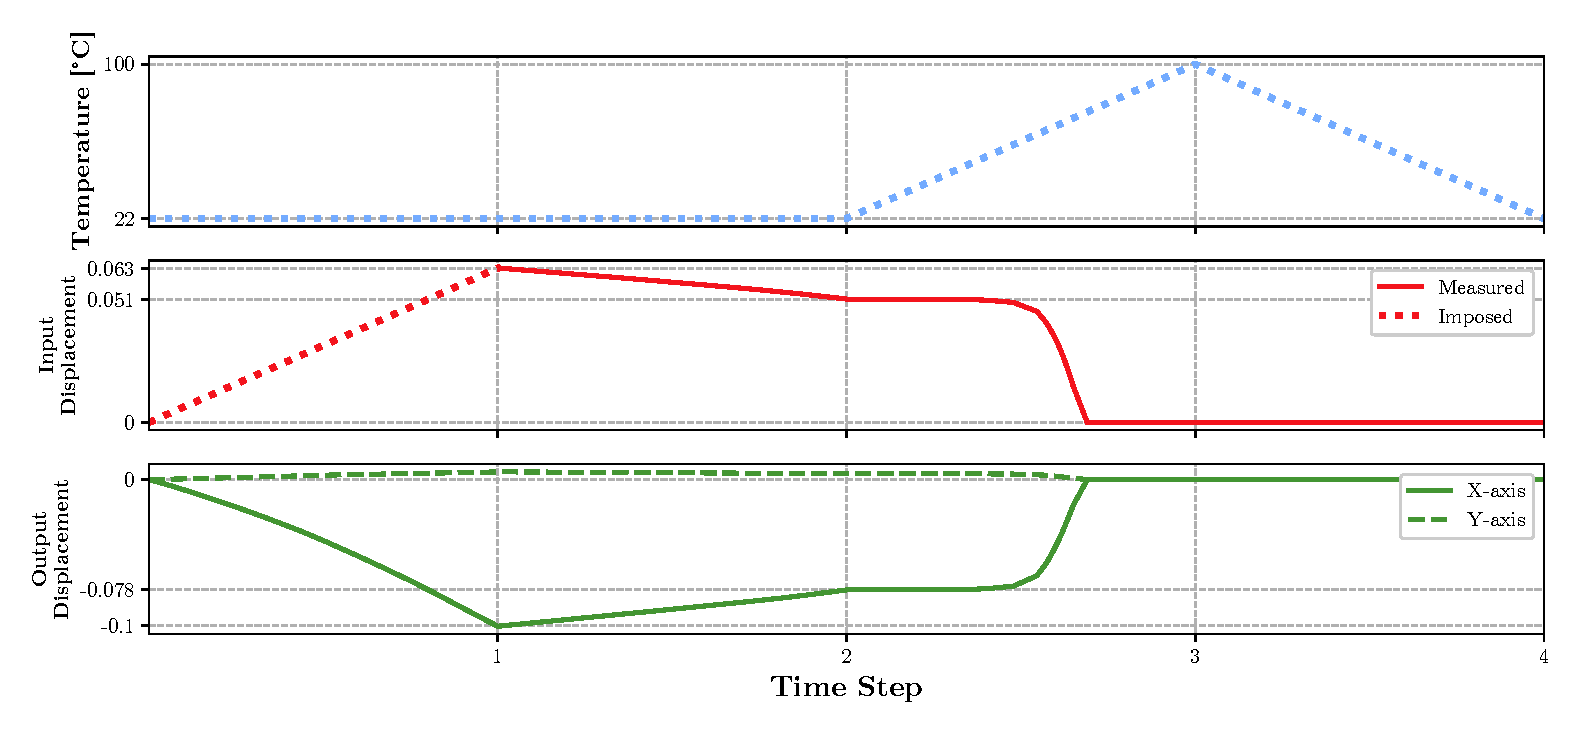
\includegraphics[width=\textwidth]{images/chap5/BM_Inverter30.eps}};
    \begin{scope}[x={(graph.south east)},y={(graph.north west)}]
    % \coordinate (ts0) at (1.54,7.6);
    % \coordinate (ts4) at (17.55,7.6);
    \coordinate (ts0) at (0.085,0.945);
    \coordinate (ts4) at (0.985,0.945);
    \coordinate (ts1) at ($ (ts0)!0.25!(ts4) $);
    \coordinate (ts2) at ($ (ts0)!0.5!(ts4) $);
    \coordinate (ts3) at ($ (ts0)!0.75!(ts4) $);
    \node[anchor=mid,inner sep=0] (ls0) at ($(ts0)!0.5!(ts1) + (0,0.05) $) {\fbox{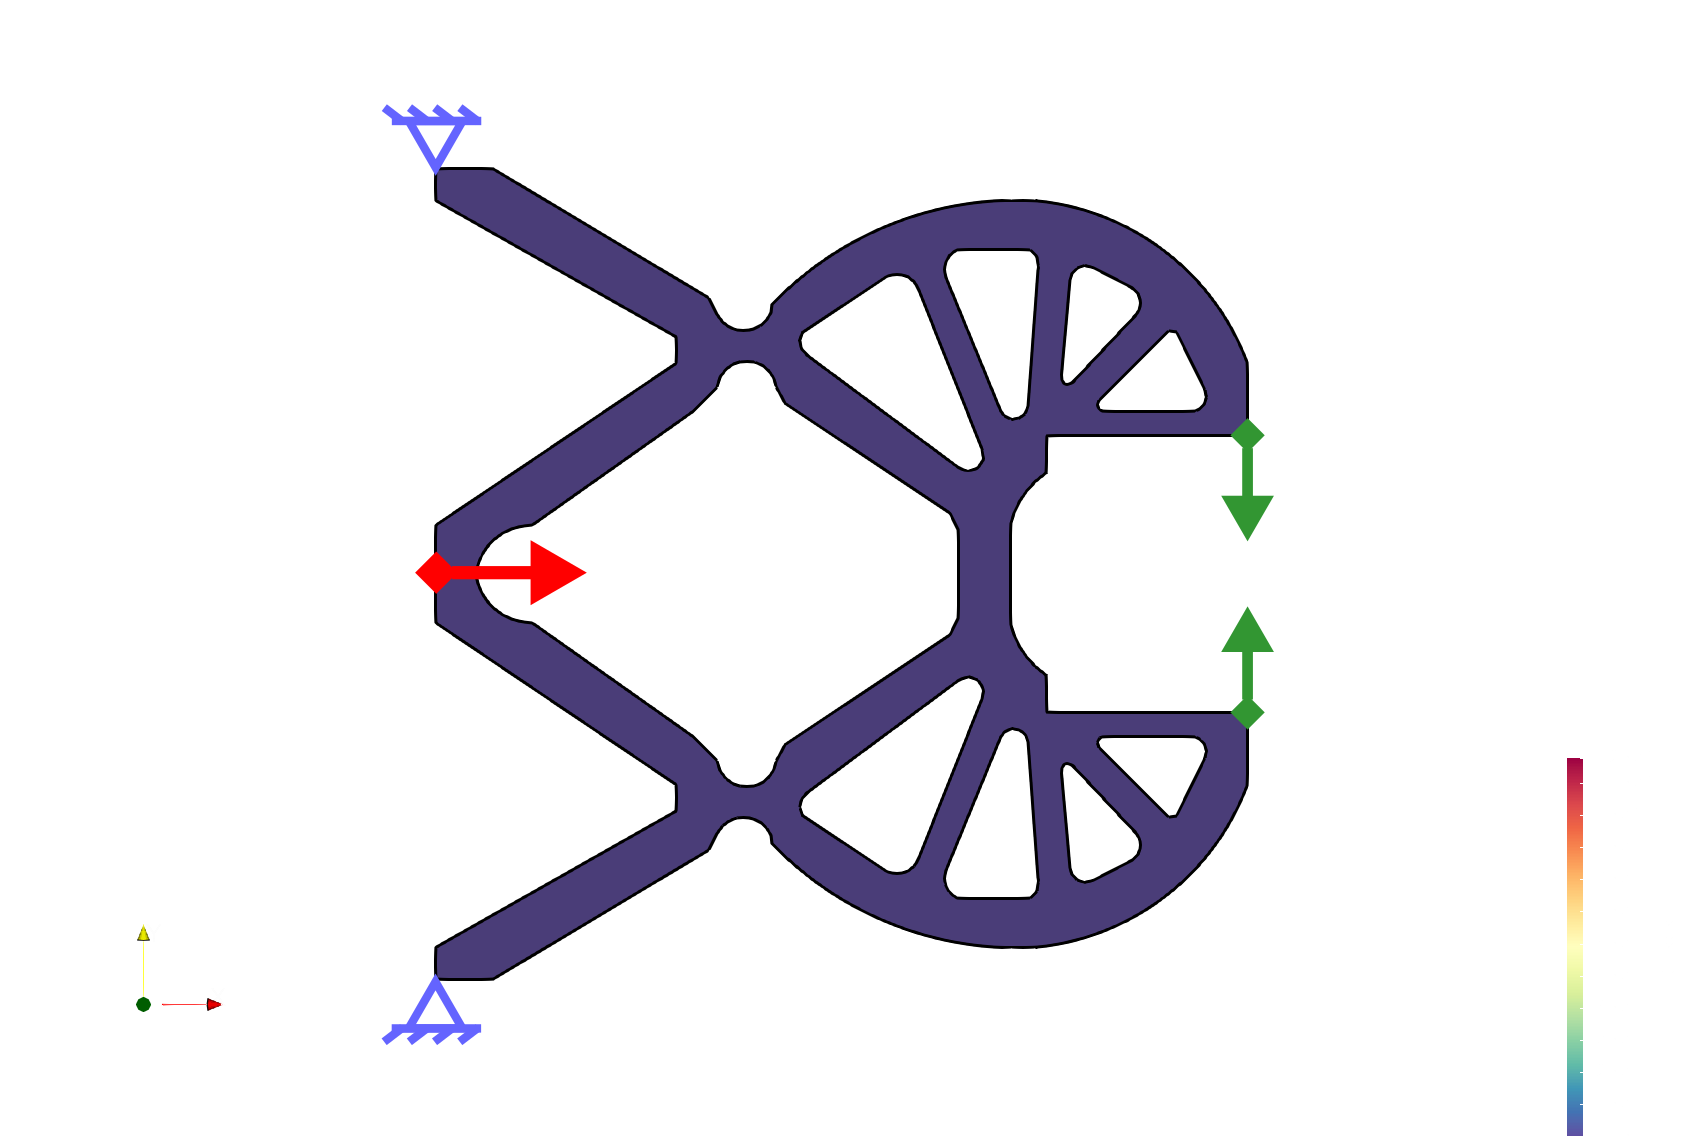
\includegraphics[height = 2cm,trim={11cm 3cm 13cm 3cm},clip]{images/chap5/Gripper_step0_v3.png}}};
    \draw[black, thick, -latex](ls0.west) to [bend right] (ts0);
    \node[anchor=mid,inner sep=0] (ls1) at ($(ts1)!0.5!(ts2) + (0,0.05) $) {\fbox{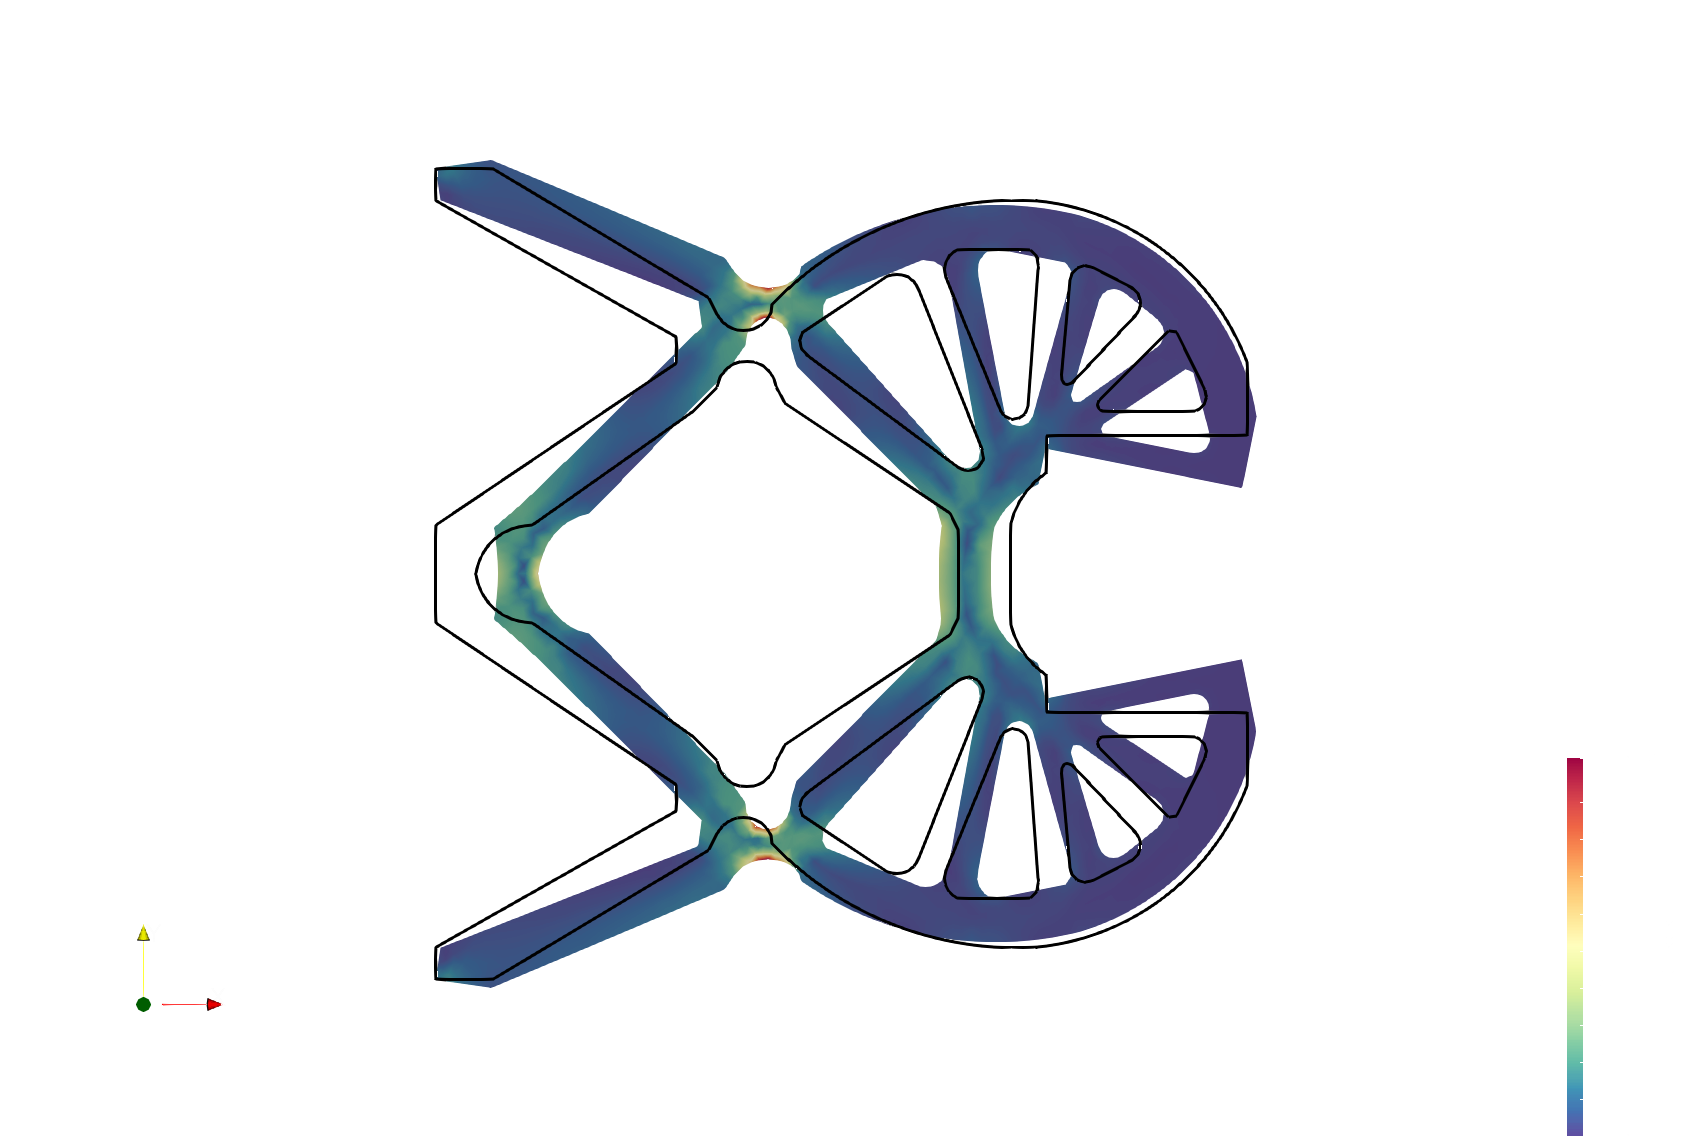
\includegraphics[height = 2cm,trim={11cm 3cm 13cm 3cm},clip]{images/chap5/Gripper_step1.png}}};
    \draw[black, thick, -latex](ls1.west) to [bend right] (ts1);
    \node[anchor=mid,inner sep=0] (ls2) at ($(ts2)!0.5!(ts3) + (0,0.05) $) {\fbox{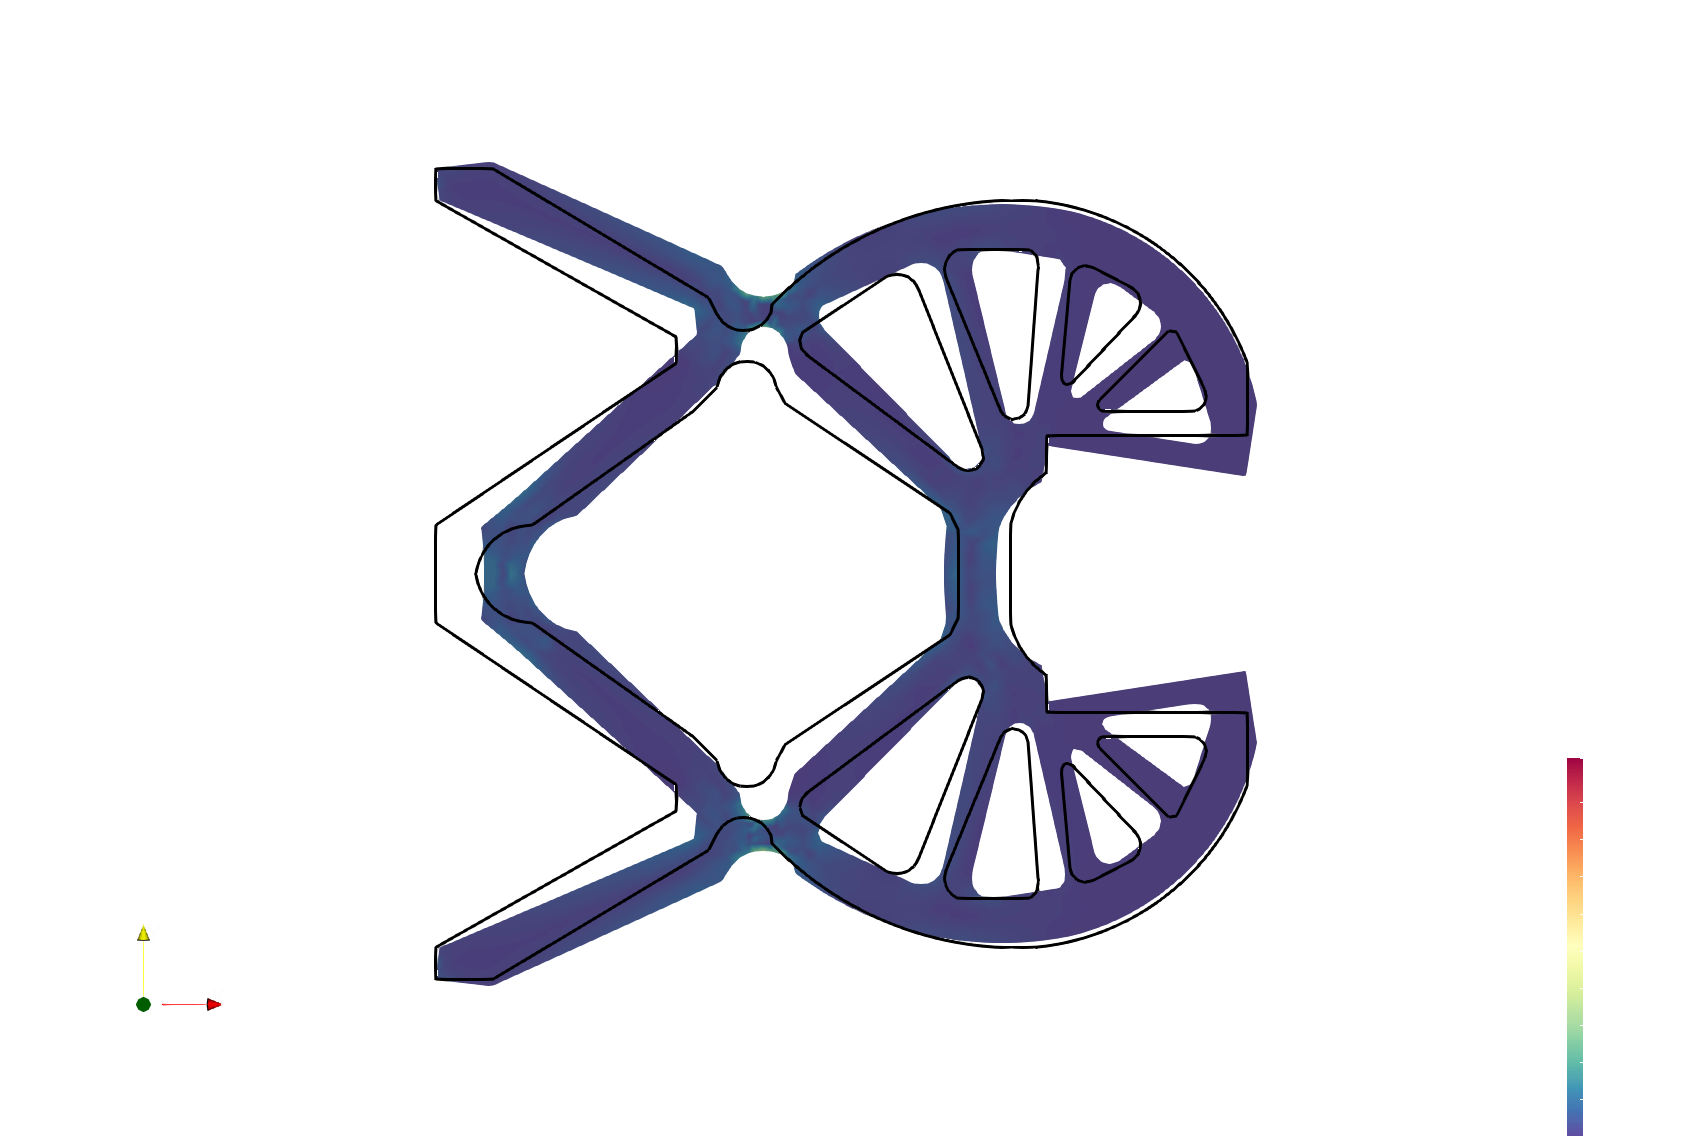
\includegraphics[height = 2cm,trim={11cm 3cm 13cm 3cm},clip]{images/chap5/Gripper_step2.png}}};
    \draw[black, thick, -latex](ls2.west) to [bend right] (ts2);
    \node[anchor=mid,inner sep=0] (ls3) at ($(ts3)!0.5!(ts4) + (0,0.05) $) {\fbox{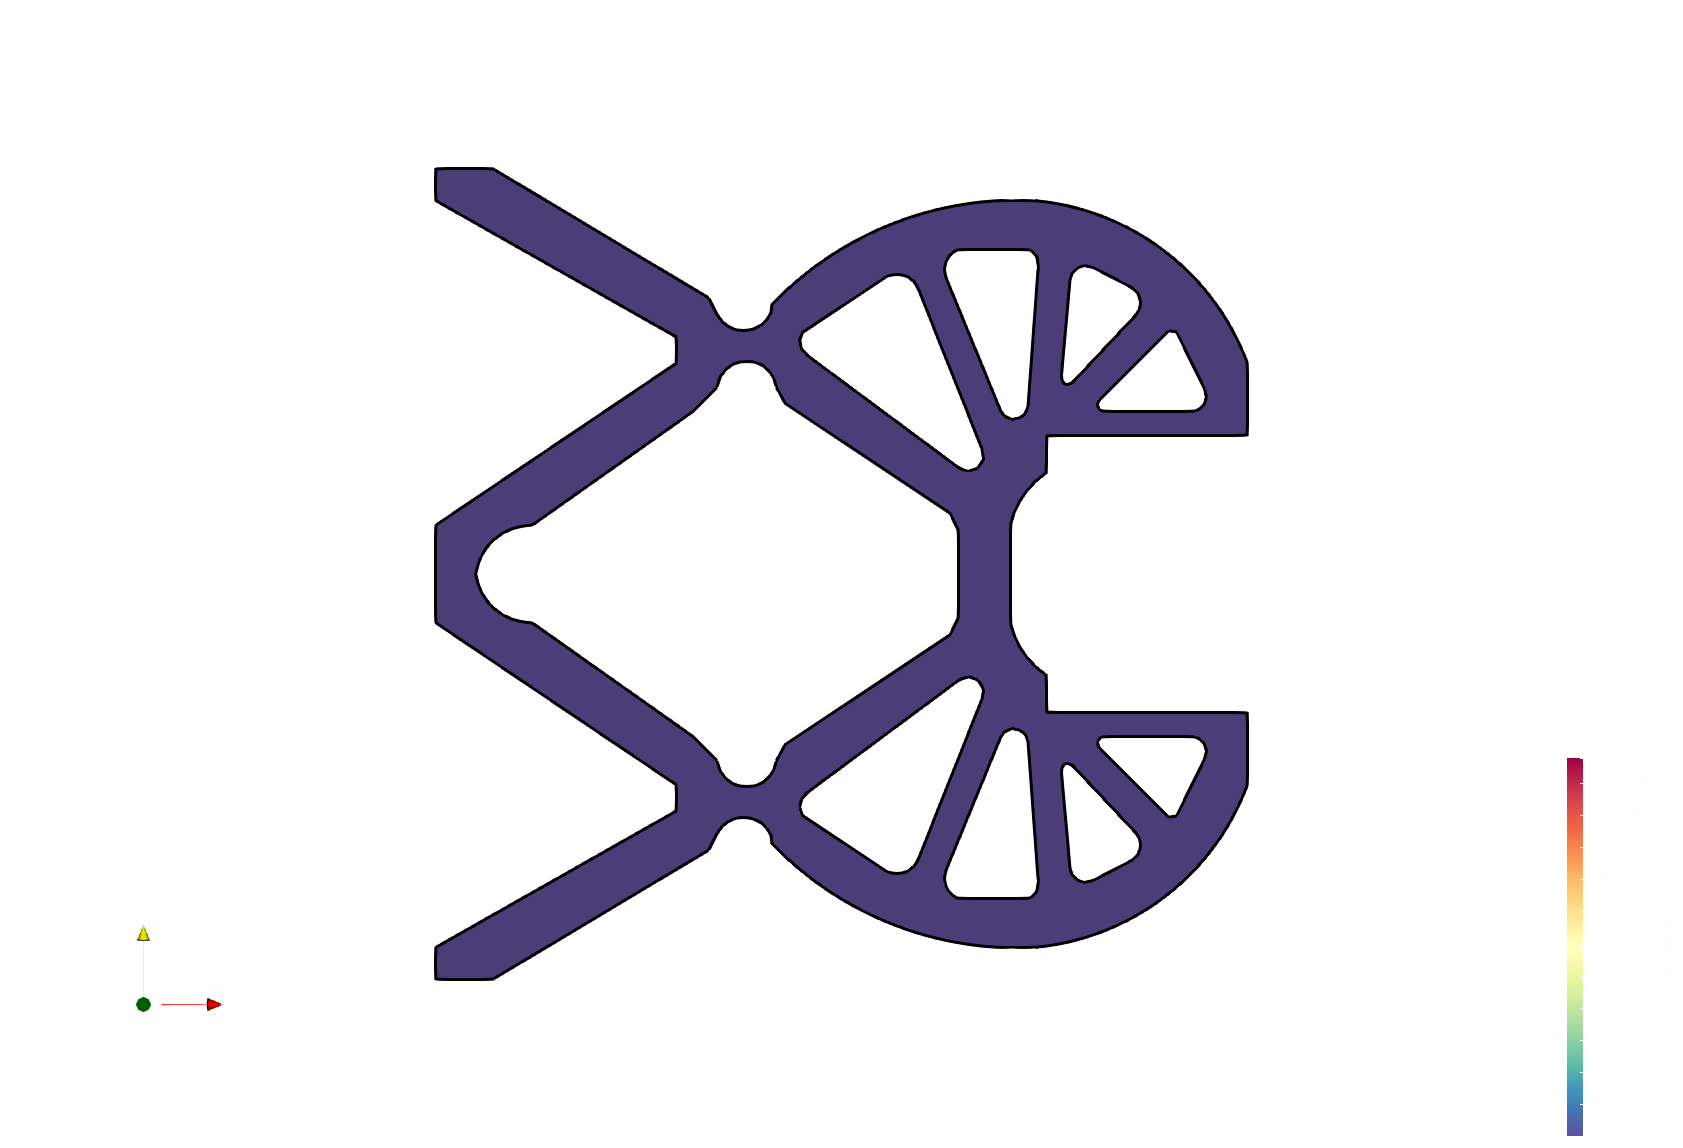
\includegraphics[height = 2cm,trim={11cm 3cm 13cm 3cm},clip]{images/chap5/Gripper_step0.png}}};
    \draw[black, thick, -latex](ls3.west) to [bend right] (ts3);
    \node[anchor=south east,inner sep=0] (ls0) at ($(ts4) + (0,0.015) $) {
\includegraphics[height = 2.3cm]{images/chap5/Colorbar.pdf}};
    \end{scope}
    \end{tikzpicture}%
\end{document}
